% !TeX encoding = UTF-8
% !TeX program = xelatex
% !TeX spellcheck = fr
\documentclass[11pt,a4paper]{report}
\usepackage{styles/preambule_college}
\usepackage{styles/preambule_personnalisation}
\usepackage[version=4]{mhchem}
%\setcounter{tocdepth}{3}

\includeonly{tm_astro_chap01,tm_astro_chap02,tm_astro_chap03,tm_astro_chap04,tm_astro_chap05,tm_astro_appendix}

\begin{document}

\tableofcontents

\chapterFormat

% !TeX encoding = UTF-8
% !TeX program = xelatex
% !TeX spellcheck = fr
% !TeX root = tm_astro_main.tex



\chapter{Structure interne des étoiles}
% !TeX encoding = UTF-8
% !TeX program = xelatex
% !TeX spellcheck = fr
% !TeX root = tm_astro_main.tex


	
\chapter{Evolution stellaire}\label{2}

\section{La séquence principale}\label{2.1}

Lorsqu’une étoile s’est formée, des réactions nucléaires commencent à s’amorcer dans son cœur sous l’effet de la pression engendrée par la force gravitationnelle. Ces réactions qui peuvent durer plusieurs milliards d’années consistent principalement à fusionner de l’hydrogène en hélium. Il existe deux processus pour arriver à cela : la chaîne proton-proton et le cycle Carbone-Azote-Oxygène.

\subsection{La chaîne proton-proton}\label{2.1.1}


\begin{equation}\ce{\ce{1H} + \ce{1H} -> \ce{2D} + \ce{e+} + $\nu_{e}$}\label{Eq. 2.1}\end{equation}
\begin{equation}\ce{\ce{2D} + \ce{1H} -> \ce{3He} + g}\label{Eq. 2.2}\end{equation}
\begin{equation}\ce{\ce{3He} + \ce{3He} -> \ce{4He} + \ce{21H}}\label{Eq. 2.3}\end{equation}\smallskip	


La fusion de l’hydrogène ne fait pas que de produire de l’hélium, elle libère aussi beaucoup d’énergie. Ce processus crée une pression qui est capable de compenser la compression gravitationnelle et ainsi permet d’équilibrer thermodynamiquement l’étoile (§\ref{1}).
Nous pouvons expliquer la longévité de cette phase de vie d’une étoile par la lenteur de la réaction (Eq. \ref{Eq. 2.1}). En effet, l’Eq. \ref{Eq. 2.1} décrit une interaction faible qui est par définition extrêmement lente à cause de sa faible section efficace (probabilité qu’une interaction de type faible se produise).

\subsection{Le cycle CNO}\label{2.1.2}

Les étoiles composées de gaz enrichis de plusieurs générations stellaires possèdent déjà des éléments lourds comme le carbone, l’azote ou bien encore l’oxygène dans leur composition. Ces éléments servent de très bons catalyseurs pour créer de l’hélium.


\begin{equation}\ce{\ce{12C} + \ce{1H} -> \ce{13N} +$\gamma$}\label{Eq. 2.4}\end{equation}				     	
\begin{equation}\ce{\ce{13N} -> \ce{13C} + \ce{e+} + $\nu_{e}$ }\label{Eq. 2.5}\end{equation}					   	
\begin{equation}\ce{\ce{13C} + \ce{1H} -> \ce{14N} + $\gamma$ }\label{Eq. 2.6}\end{equation}	
\begin{equation}\ce{\ce{14N} + \ce{1H} -> \ce{15O} + $\gamma$}\label{Eq. 2.7}\end{equation}\newpage\vspace{2cm}		
\begin{equation}\ce{\ce{15O} -> \ce{15N} + \ce{e+} + $\nu_{e}$	}\label{Eq. 2.8}\end{equation}
\begin{equation}\ce{\ce{15N} + \ce{1H} -> \ce{12C} + \ce{4He}}\label{Eq. 2.9}\end{equation}\smallskip

\begin{figure}[H]
	\centering
	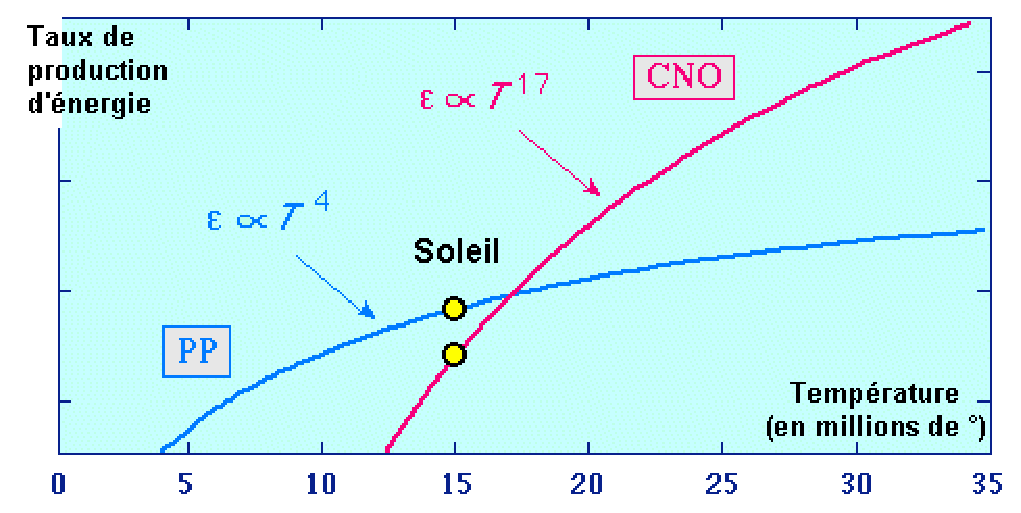
\includegraphics[scale=0.8]{images/cno-pp}
	\caption[Comparaison des cycles PP et CNO\newline\url{http://nrumiano.free.fr/Fetoiles/energie.html}]{Comparaison des cycles PP et CNO}
	\label{Fig. 2.1}
\end{figure}\bigskip

Le graphique ci-dessus nous montre que la chaîne proton-proton reste la principale source d’énergie des étoiles allant jusqu’à 2 $M_\odot$. Dans les étoiles de ce type, l’énergie est transmise de manière radiative dans le cœur, tandis que dans les couches supérieures, c’est la convection qui la transporte. Lorsque les 2 $M_\odot$ sont dépassées, le cycle CNO devient plus fréquent que la chaîne proton-proton. Cette limite franchie, les couches intérieures de l’étoile reçoivent leur énergie plutôt de manière convective, alors que les couches supérieures la reçoive par radiation.

\subsection{Le diagramme de Hertzsprung-Russell}\label{2.1.3}

Même si toutes les étoiles sont soumises à ces cycles de production de l’hélium, elles ne sont pas toutes les mêmes. Elles se distinguent notamment par des différences de luminosité, de types spectrales (couleurs) ou bien encore de masse. Ce diagramme (Fig. \ref{Fig. 2.2}), nommé d’après ses créateurs, représente des populations d’étoiles classées selon leur luminosité et leur type spectrale. La masse n’est pas représentée comme l’un des axes car elle est étroitement liée à la luminosité de l’étoile (Eq. \ref{Eq. 2.10}).

\begin{equation}L \propto M^{3}\label{Eq. 2.10}\end{equation}\newpage

\begin{figure}[H]\vspace{1cm}
	\centering
	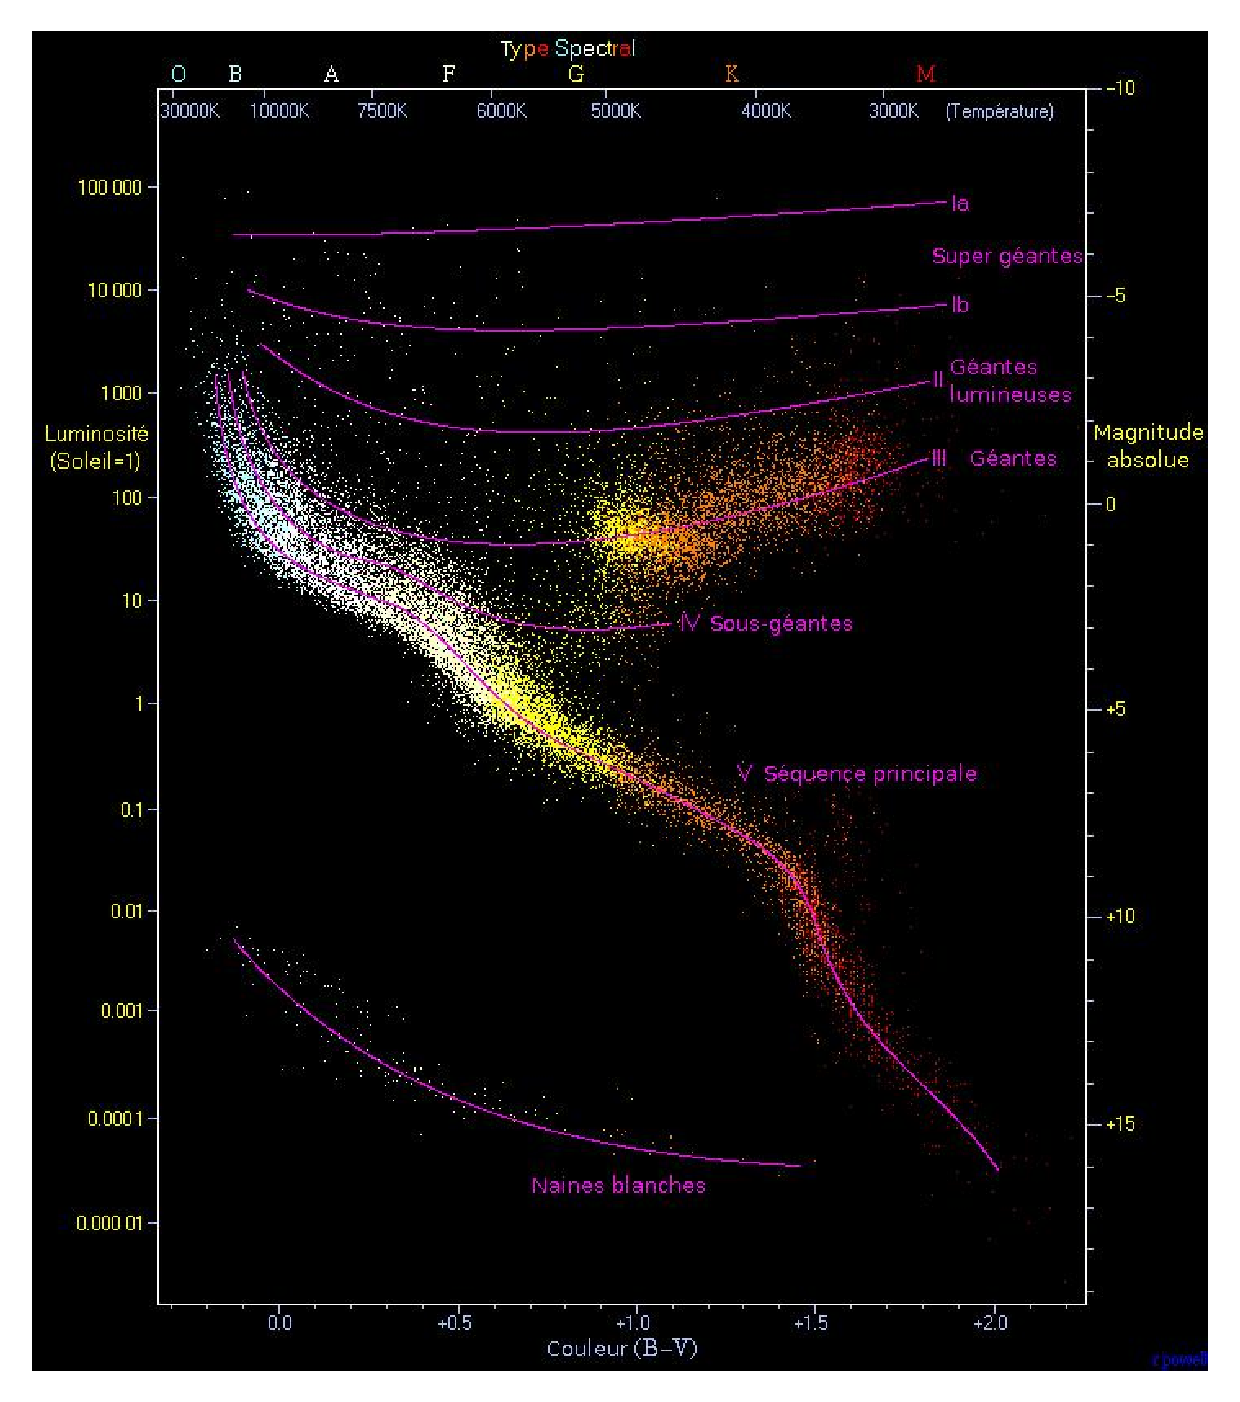
\includegraphics[scale=0.4]{images/hr-diagram}
	\caption[Diagramme de Hertzsprung-Russell\newline\url{http://www.astrosurf.com/luxorion/vie-etoiles2.html}]{Diagramme de Hertzsprung-Russell}
	\label{Fig. 2.2}
\end{figure}\bigskip

Nous pouvons facilement distinguer que certaines zones bien précises se délimitent, elles représentent les différents types d’étoiles. De plus, tout au long de sa vie une étoile se déplace dans ce diagramme. Par exemple, le soleil achèvera son existence dans la branche des naines blanches. Le diagramme HR représente l’un des outils les plus importants de l’astrophysique moderne, car il permet de prédire l’emplacement d’une étoile et en suite de le comparer avec les observations effectuées sur ce même objet.\bigskip

\section{La phase géante rouge}\label{2.2}

Les réserves d’hydrogène d’une étoile ne sont pas illimitées. En effet, il arrive un moment où il n’y a plus assez d’hydrogène dans le cœur de l’étoile pour entretenir les fusions nucléaires, la pression engendrée par ces réactions disparaît et donc l’équilibre hydrostatique est rompu. Le cœur, alors principalement composé d’hélium, ne possède pas la température nécessaire pour débuter la fusion de l’hélium ($10^{8}$ K), il se contracte alors à cause de la pression gravitationnelle. Sous l’effet de cette contraction, l’enveloppe d’hydrogène entourant le noyau atteint une température suffisante pour réamorcer la fusion nucléaire. L’agrandissement du rayon de l’étoile s’explique de deux manières différentes :

\begin{figure}[H]\vspace{1cm}
	\centering
	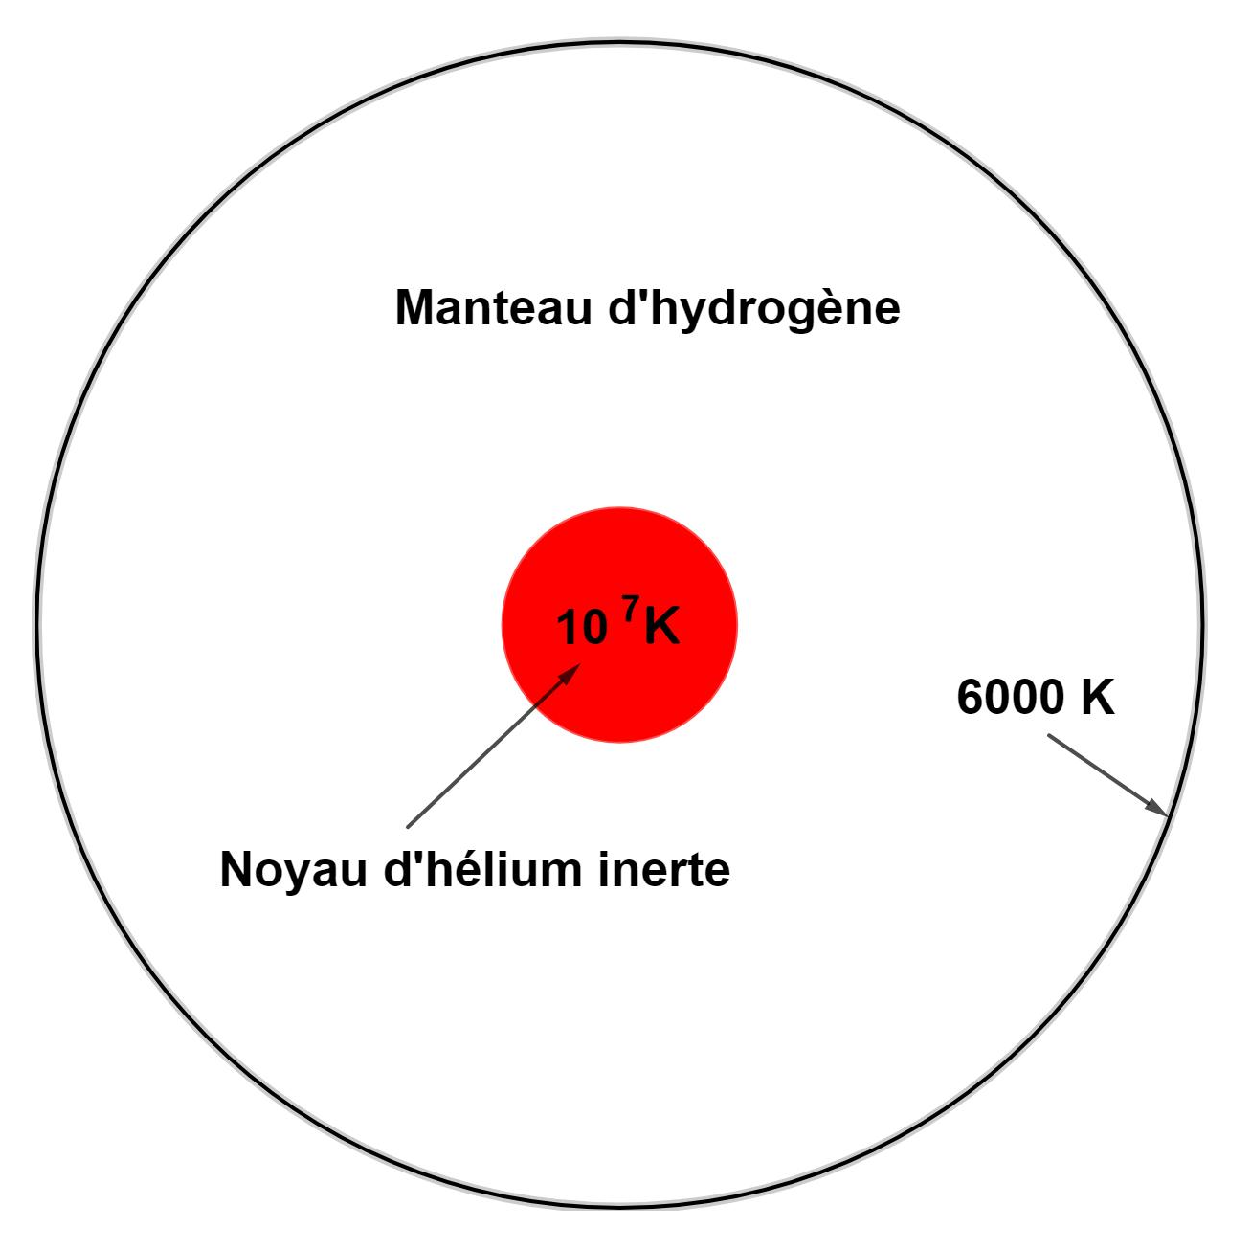
\includegraphics[scale=0.45]{images/compo_sp}
	\caption[Composition d'une étoile (soleil) à la fin de la séquence principale -figure réalisée avec GeoGebra]{Composition d'une étoile (soleil) à la fin de la séquence principale}
	\label{Fig. 2.3}
\end{figure}\bigskip                         

\begin{enumerate}
	\item L’énergie produite par la fusion en couche de l’hydrogène réchauffe et donc dilate l’enveloppe stellaire.
	\item La contraction du noyau de l’étoile est stoppée par la pression de dégénérescence des électrons (annexe). Cette pression d’origine quantique découle tout droit du principe d’exclusion de Pauli (deux électrons ne peuvent pas se trouver dans le même état quantique). Autrement dit, il existe une pression limite que nous ne pouvons pas franchir car toutes les couches électroniques de basses énergies d’un atome sont occupées. Lorsque cette limite est atteinte, l’énergie associée à la compression gravitationnelle se transforme en énergie thermique. La température du cœur va alors augmenter drastiquement, sans que pour autant la pression ne varie, et ainsi dilater les couches extérieures de l’étoile qui, elles, vont diminuer de température, d’où la couleur rouge, orange qui correspond à une plus faible température. 
	
\end{enumerate}

\subsection{Flash de l'hélium}\label{2.2.1}

Pour les étoiles comprises entre 0,5 et 2 $M_\odot$, il existe un phénomène extrêmement puissant qui se produit lorsque le cœur de l’étoile atteint les $10^{8}$ K, température nécessaire pour amorcer la fusion de l’hélium. En quelques instants, tout le noyau de l’étoile enclenche la fusion de l’hélium en carbone (réaction triple alpha). Cette explosion génère autant de luminosité que toute une galaxie, cependant la majorité de cette énergie est absorbée par le plasma de l’étoile qui se dilate fortement. Lorsque l’énergie thermique du noyau redevient inférieure à l’énergie de Fermi, son gaz n’est plus dégénéré. L’étoile se retrouve donc sur une sorte de nouvelle séquence principale (en plus court), mais cette fois-ci elle fusionne de l’hélium pour former du carbone et de l’oxygène en son centre. De plus, l’enveloppe d’hydrogène qui entoure le noyau continue aussi à former de l’hélium.\smallskip

Quant aux étoiles supérieures à 2 $M_\odot$, elles sont suffisamment massives pour atteindre les conditions requises à la réaction triple alpha sans passer par les flashs de l’hélium.\newpage

\begin{figure}[H]\vspace{1cm}
	\centering
	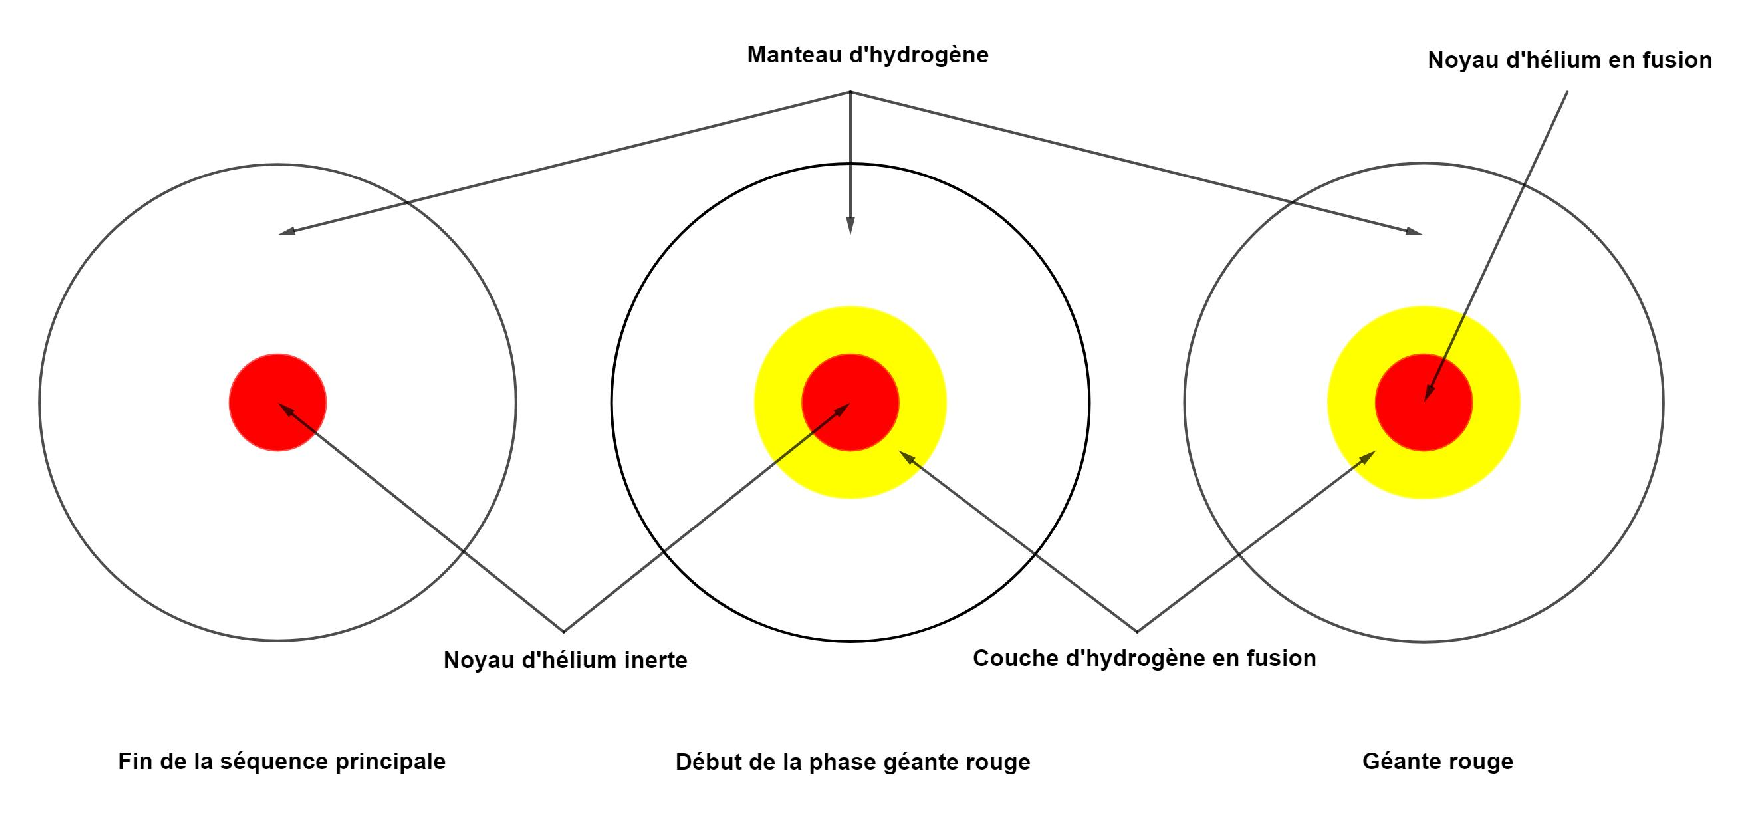
\includegraphics[scale=0.40]{images/compo_sp_gr}
	\caption[Comparaison entre les différentes premières phases de fusion d'une étoile (pas à l'échelle) - figure réalisée avec GeoGebra]{Comparaison entre les différentes premières phases de fusion d'une étoile (pas à l'échelle)}
	\label{Fig. 2.4}
\end{figure}

\subsection{AGB (branche asymptotique des géantes)}\label{2.2.2}

Une fois l’hélium épuisé dans le noyau stellaire le cycle recommence : contraction du cœur, augmentation de la température, reprise des fusions thermonucléaires dans les coquilles d’hydrogène ainsi que d’hélium. La fusion en couche de l’hydrogène et de l’hélium se révèle être très agitée. Ces couches deviennent par moment instables et créent des pulsations thermiques. Ces pulsations ont pour effet de créer des vents stellaires qui font perdre de la masse à l’étoile.

\section{Les naines blanches}\label{2.3}

Les étoiles sont sujettes à expulser d’énormes quantités de masses à cause des vents stellaires. Les étoiles, allant jusqu’à 9 $M_\odot$, se retrouvent avec des masses situées entre 0,6 et 1,1 $M_\odot$ sous l’effet de ces vents. Ces étoiles sont destinées à devenir des naines blanches car elles se trouvent en-dessous de la masse de Chandrasekhar (1,44 $M_\odot$) (annexe). La matière est éjectée de l’étoile de manière symétrique, ainsi se forme une enveloppe, appelée circumstellaire, tout autour du centre de l’étoile. Il ne reste donc plus que le noyau de l’étoile composé d’oxygène et de carbone. Du fait de l’arrêt des réactions thermodynamiques, le centre se contracte jusqu’à ce qu’il s’équilibre une nouvelle fois grâce à la pression de dégénérescence des électrons. Le rayon moyen des naines blanches correspond plus ou moins à celui de la Terre. Cependant, elles possèdent une masse similaire à celle du Soleil, qui possède un rayon 109 fois supérieur à celui de la Terre (Fig. \ref{Fig. 2.3}). De plus, l’enveloppe circumstellaire est illuminée pendant des milliards d’année par la naine blanche en son sein qui se refroidit gentiment, on appelle cela une nébuleuse planétaire. Ces nébuleuses n’ont rien à voir avec des planètes, elles sont historiquement nommées ainsi du fait de leur apparence qui peut faire penser à une planète.\newpage 

\begin{figure}[H]\vspace{1cm}
	\centering
	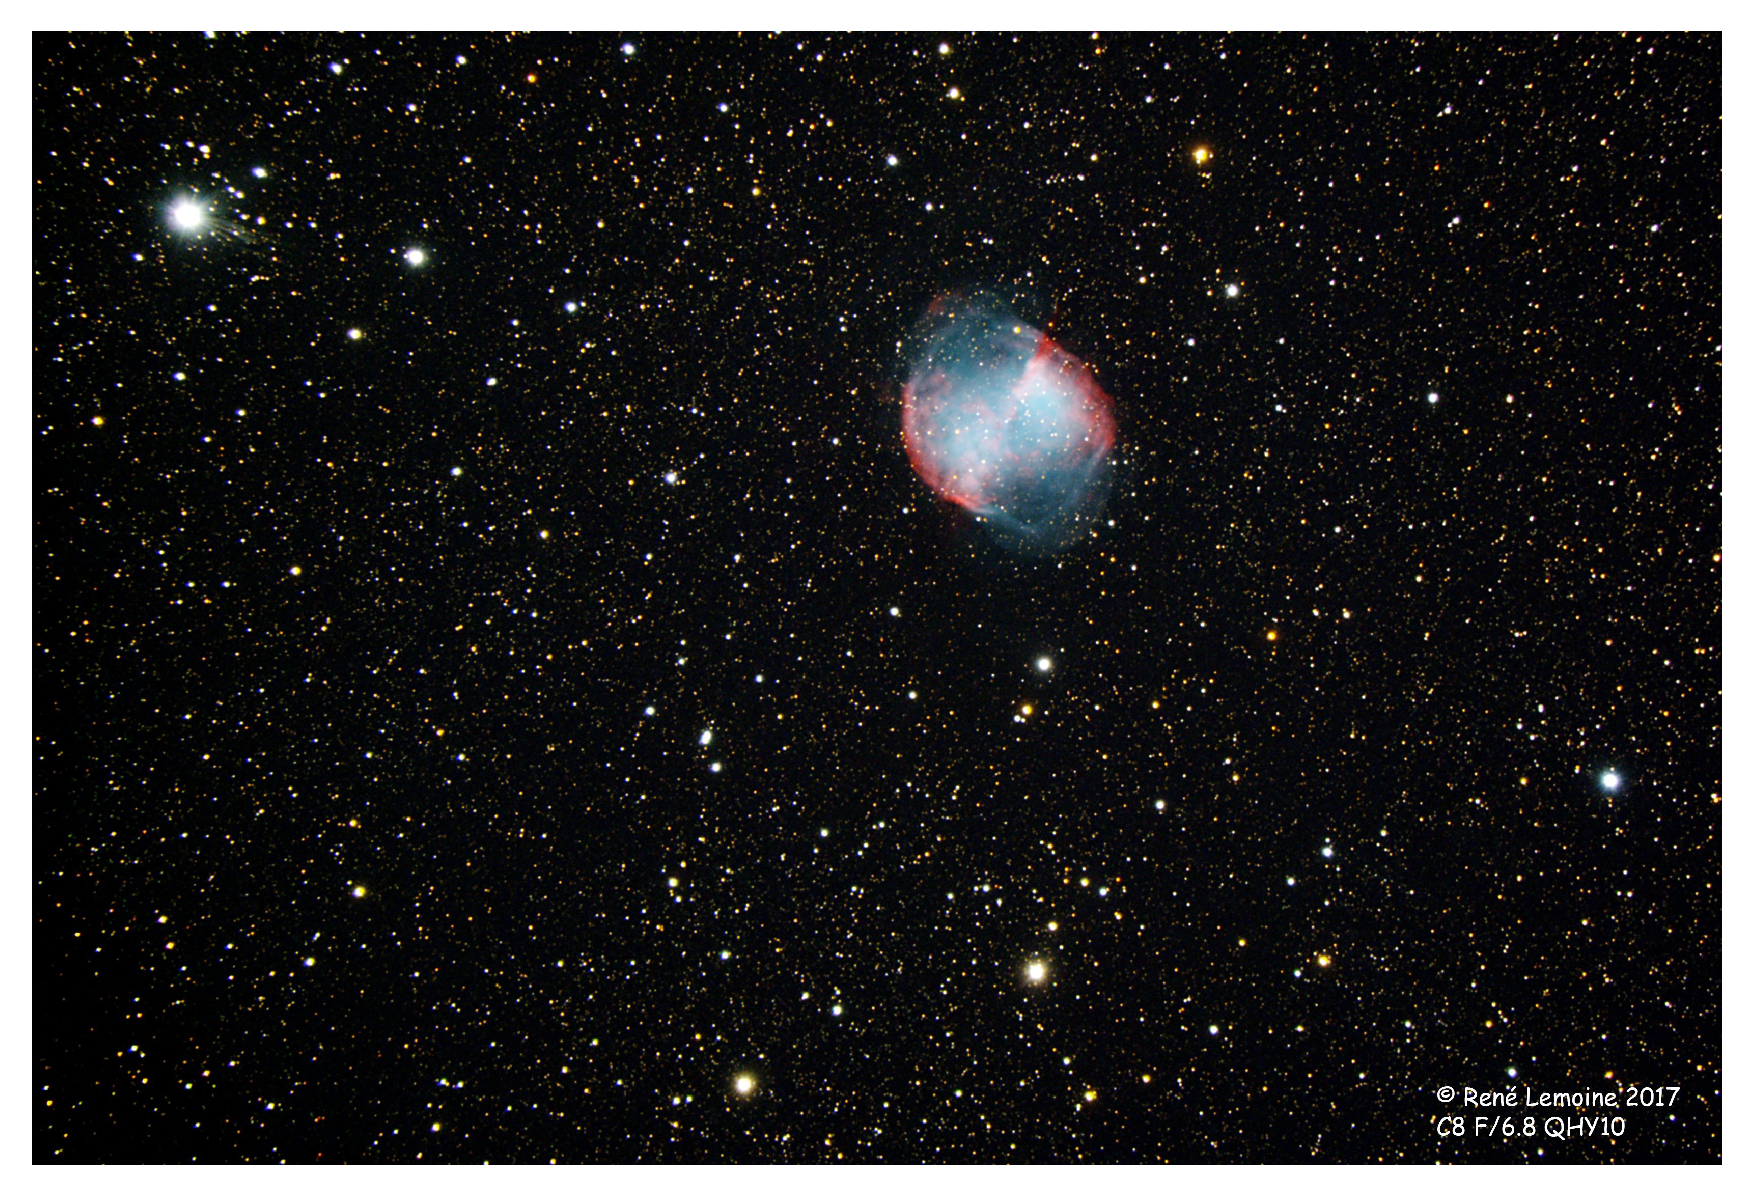
\includegraphics[scale=0.4]{images/m27}
	\caption[M27, nébuleuse planétaire de l'haltère - astrophoto prise par René Lemoine le 30 juillet 2017 avec un Celestron 8 (1h50 de pose)]{M27, nébuleuse planétaire de l'haltère}
	\label{Fig. 2.5}
\end{figure}  

\section{Evolution tardive des étoiles massives}\label{2.4}

Les étoiles de plus de 9 $M_\odot$ ne s’arrêtent pas à la fusion de l’oxygène et du carbone. En effet, leur grande masse leurs permettent d’atteindre de plus grandes échelles de pressions et de températures, ce qui leur permettent de produire des éléments plus lourds comme le magnésium, le néon, le souffre, le silicium ou bien encore le fer. Ces atomes sont produits de manière analogue au carbone et à l’oxygène mais avec des réactions plus complexes. Une des principales caractéristiques de ces étoiles massive est que leur gaz n’est jamais dégénéré (soumis à la pression de dégénérescence des électrons) jusqu’à leur dernier stade d’évolution, lorsque le noyau est constitué de fer. La nucléosynthèse par fusion s’arrête obligatoirement au fer. En effet, le rendement énergétique des réactions de fusion décroit lorsque la masse de l’atome augmente, et c’est à partir de l’élément fer que ces réactions de fusions qui étaient exothermiques, deviennent endothermiques. A ce stade, on dit que l’étoile, appelée supergéante, possède une structure en pelures d’oignon (Fig. \ref{Fig. 2.6}).

\begin{figure}[H]
	\centering
	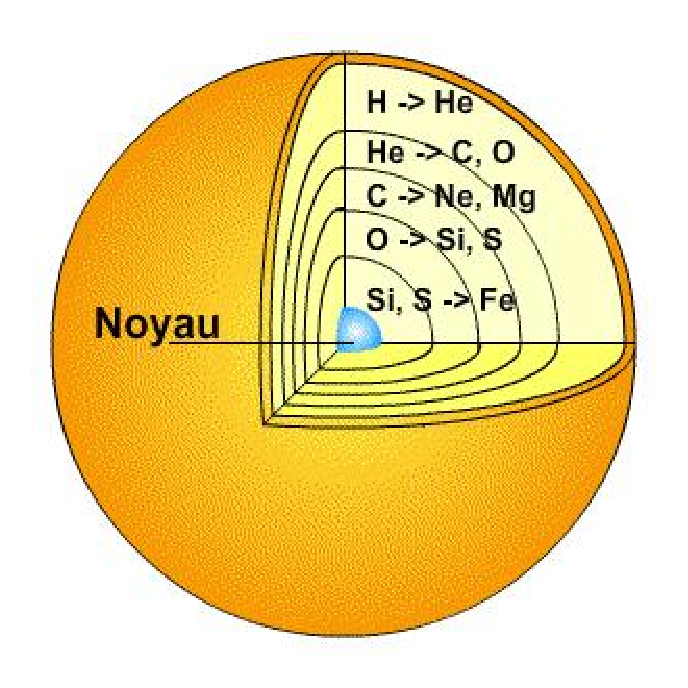
\includegraphics[scale=0.3]{images/oignon}
	\caption[Structure en pelures d'oignon d'une supergéante\newline \url{https://media4.obspm.fr/public/ressources\_lu/pages\_vie-mort/impression.html}]{Structure en pelures d'oignon d'une supergéante}
	\label{Fig. 2.6}
\end{figure}\newpage

Lorsque les réactions thermonucléaires prennent fin dans le cœur de l’étoile, ce dernier se contracte brutalement. Même la pression de dégénérescence des électrons ne suffit pas à compenser la pression gravitationnelle. Les protons capturent les électrons pour ne former plus que des neutrons. Cet effondrement, qui ne dure que quelques secondes, produit une onde de choc pulvérisant la supergéante. Ce phénomène est désigné par le terme de supernova de type II (§\ref{3.1.1}). Il ne reste de cette explosion que le cœur composé de fer. En fonction de sa masse, il deviendra soit une étoile à neutrons soit un trou noir. De plus, toute la matière éjectée forme ce qu’on l’on appelle, le rémanent de la supernova. Les différents types des supernovas seront plus détaillés au chapitre 3 (§\ref{3}).

\begin{figure}[H]
	\centering
	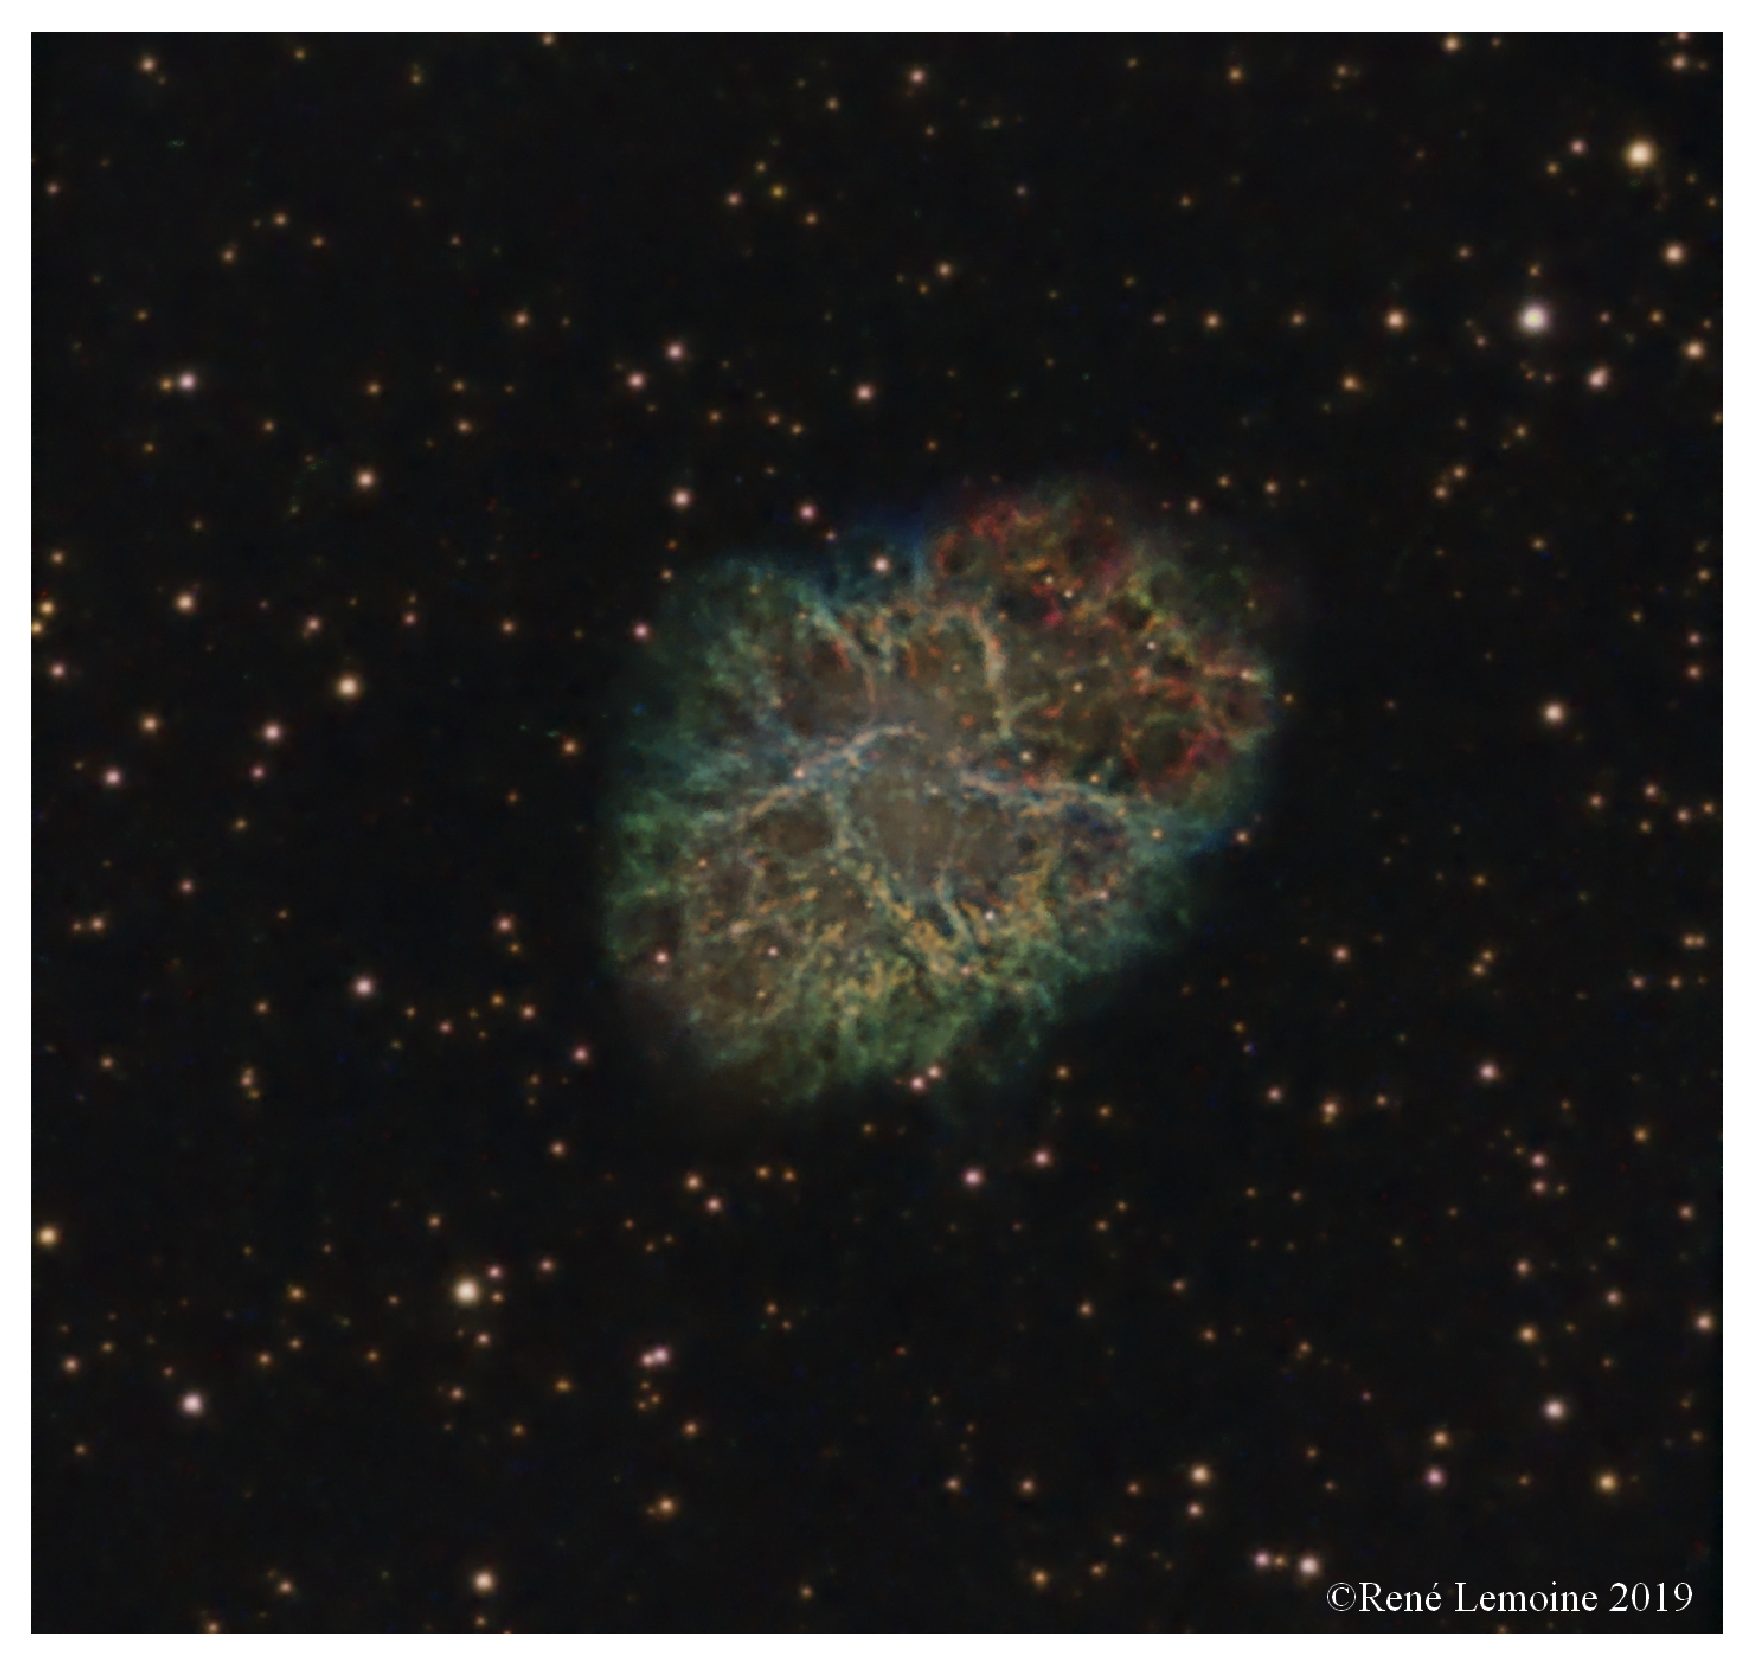
\includegraphics[scale=0.3]{images/m1}
	\caption[M1, nébuleuse du Crabe - astrophoto prise par René Lemoine le 29 janvier 2019 avec un Celestron 8 (6h de pose)]{M1, nébuleuse du Crabe, rémanent d'une supernova datant de 1054}
	\label{Fig. 2.7}
\end{figure}

A titre de comparaison, la nébuleuse de la Fig. \ref{Fig. 2.5} s'étend sur 1,44 années-lumière, tandis que le rémanent de supernova de la Fig. \ref{Fig. 2.7} mesure 5,5 années-lumière. Ces tailles démesurées témoignent de la violence de la mort d'une étoile, que ce soit par explosion en nébuleuse planétaire (§\ref{2.3}) ou par supernova (§\ref{3}). 

\section{Tableau récapitulatif de la nucléosynthèse stellaire}\label{2.5}



% !TeX encoding = UTF-8
% !TeX program = xelatex
% !TeX spellcheck = fr
% !TeX root = tm_astro_main.tex


\chapter{Supernovas}

Les étoiles dépassant 9 $M_\odot$ produisent obligatoirement une supernova au terme de leur vie (§2). Ces explosions, qui peuvent atteindre des luminosités équivalentes à 1 milliard de soleils, éjectent leur matière à quelques fractions de la vitesse de la lumière. En effet, la supernova relâche une quantité d'énergie, sous forme cinétique, égale à 1 Bethe. 1 Bethe correspond à $10^{44}$J; cette unité a été nommée en l'honneur de Hans Bethe pour ses travaux sur les supernovas. A titre de comparaison, la bombe Tsar, plus puissante bombe nucléaire jamais utilisée, dégagea une énergie de $10^{17}$J, ce qui est $10^{27}$ fois moins fort que l'énergie cinétique d'une supernova. %comparaison avec masse énergie totale de la Terre ?%
Cependant, toutes les supernovas ne sont pas causées par l'effondrement gravitationnelle d'une étoile massive (§2), il existe d'autres processus qui permettent d'aboutir à de telles explosions.\bigskip

\section{Types de supernovas} \medskip

Les supernovas ont été historiquement classées selon leur spectre électromagnétique. Si l'on détecte de l'hydrogène dans l'explosion, alors la supernova est de type II. A l'opposé, si l'on en détecte pas, alors la supernova est de type I. Cependant, cette classification ne tient pas compte de l'origine du phénomène, c'est pourquoi des subdivisons supplémentaires ont été crées afin de tenir compte d'autres critères. Les supernovas résultant d'un effondrement gravitationnel d'une étoile massive sont appelées supernovas à effondrement de cœur et sont classées dans les type Ib, Ic et II (§3.1.1). Le groupe Ia correspond aux supernovas appelées thermonucléaires. Ces-dernières sont causées par une naine blanche accrétant de la matière à une étoile proche (§3.1.2).\bigskip

\subsection{Supernovas à effondrement gravitationnelle }\medskip

Les supernovas à effondrement gravitationnelle marquent la fin de vie des étoiles dont la masse est supérieure à 9 $M_\odot$. Ces étoiles possèdent un noyau en fer, entouré par des couches de différentes compositions (Fig. 2.6). Comme plus aucune réaction nucléaire n'a lieu dans le cœur (§2.4), celui-ci commence donc à se contracter. Seul la pression de dégénérescence permet de freiner cette contraction, seulement, lorsque le noyau dégénéré dépasse la masse de Chandrasekhar (1,46 $M_\odot$), le cœur poursuit sa contraction. Du fait que le gaz est dégénéré, la température peut monter extrêmement rapidement sans occasionner des changements de pression. A partir de $10^{9}$K, la température est suffisante pour déclencher la photodésintégration du fer.\bigskip  % note de bas de page sur temp min/max %

\begin{equation} \ce{\ce{^{56}Fe} -> \ce{13\ce{^{4}He}} + \ce{4n} - {124Mev}}\end{equation}\bigskip

Cette réaction hautement endothermique, favorisant la contraction du cœur, décompose le fer en hélium et en neutrons. De plus, les photons, de plus en plus énergétique sous l'effet de la pression, deviennent capable de briser l'hélium en protons et en neutrons. La pression devient telle que les électrons sont capturés par les protons dans un processus qui s'appelle la neutronisation.\bigskip

\begin{equation} \ce{p + e{^-} -> n + $\nu$}\end{equation}\bigskip

Ce processus diminue le nombre d'électrons et par extension, la pression de dégénérescence des électrons; l'effondrement est encore une fois favorisé. Comme il ne reste bientôt plus que des neutrons, de manière analogue aux électrons, une pression de dégénérescence liée aux neutrons se crée. Cette-fois ci, la contraction  peut être stoppée. La force nucléaire forte, qui lie les protons et les neutrons dans le noyau atomique, devient répulsive lorsque la pression est supérieure à la densité d'un noyau atomique, qui est de l'ordre de $10^{17}$ kg  m$^{-3}$. Ainsi, une énorme onde de choc est crée par les couches supérieures de l'étoile lorsqu'elles rebondissent contre le noyau qui est devenu répulsif.
Les neutrinos créés lors de la neutronisation, environ $10^{57}$, emportent 99\% de l'énergie de l'explosion; les 1\% restants sont répartis entre l'énergie cinétique de la matière expulsée (0,9\%) et la luminosité de l'explosion (0,1\%). Ces particules très énergétiques possèdent une masse quasiment nulle et voyagent à des vitesses proches de celle de la lumière, en plus de cela, elles n'interagissent presque pas avec la matière. Seulement, vu leur nombre élevé ($10^{57}$), une partie d'entre-eux vont chauffer les couches de l'étoile lors de leur expulsion. Aujourd'hui, nous pensons que les neutrinos sont les principaux responsables de l'explosion de la supernova.\smallskip

Les supernovas de type Ib, Ic et II se déroulent toutes selon le processus vu ci-dessus. Ce qui les différencie, c'est leur spectre ainsi que leur courbe de lumière.\bigskip

\begin{itemize}
	
	\item Type Ib: Premièrement, il se caractérise par une absence d'hydrogène dans son spectre électromagnétique, ce qui fait de lui une supernova de type I. En plus de cela, nous retrouvons de l'hélium dans sa composition. Sa courbe de lumière montre un taux de décroissance inférieure aux supernovas de type IIL.
	
	\item Type Ic: Comme le type Ib, il ne possède pas d'hydrogène dans son spectre. Cependant, nous ne trouvons non plus pas d'hélium. La raison pour laquelle l'hydrogène ou l'hélium ne font pas partie du spectre électromagnétique des types Ib et Ic est soit que l'étoile a été balayée par de forts vents stellaires, soit qu'il s'est produit un transfert de matière dans un système binaire. Pour finir, les types Ib et Ic possèdent la même courbe de lumière.
	
	\item Type II: Le type II se distingue de tout les autres grâce à la présence d'hydrogène dans son spectre électromagnétique. Lors d'observations de supernovas composées d'hydrogène (mais pas que), on a remarqué que 2 courbes de lumière bien distinctes se délimitaient. C'est pourquoi les supernovas de type II sont encore séparées en type IIL(L pour linéaire) et IIP (P pour plateau). La courbe de lumière du type IIP forme un plateau dans les premiers mois suivants la supernova, tandis que la luminosité du type IIL décroît presque linéairement.
	
\end{itemize}\newpage


\begin{figure}[H]\vspace{1cm}
	\centering
	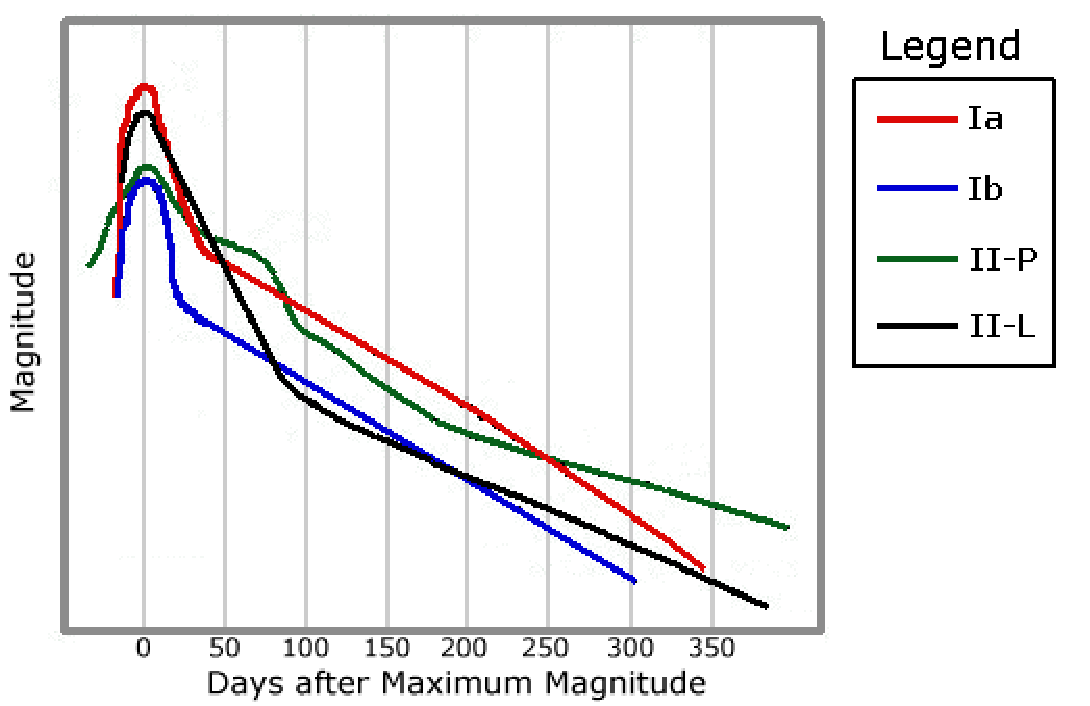
\includegraphics[scale=0.4]{images/lightcurves}
	\caption{Comparaison des courbes de lumière des différents types de supernovas}
\end{figure}\bigskip 

\subsection{Supernovas thermonucléaires}\medskip

Les supernovas thermonucléaires nécessitent un système composé d'au moins deux étoiles. Parmi ces étoiles, l'une d'entre elle doit être une naine blanche tandis que l'autre doit se situer sur la fin de la séquence principale. Pour qu'un transfert de matière puisse s'opérer, il faut que la compagne de la naine blanche dépasse son lobe de Roche. Un lobe de Roche est le volume autour d'une étoile dans lequel la matière reste en orbite autour de celle-ci, dépassé ce volume la matière quitte son orbite. De plus, il n'y a pas que la force gravitationnelle qui est prise en compte dans le calcul du lobe, la force centripète associée au système binaire l'est aussi. Si l'on projette les deux lobes sur un plan, ils forment une sorte de huit. Lorsque les couches supérieures de la géante dépassent la surface limite, il peut y avoir transfert de matière entre les étoiles. Cependant, la matière ne transite pas d'une étoile à l'autre par n'importe quel chemin, elle passe par l'intersection entre les deux lobes de Roche, le centre du huit (Fig. 3.2).\bigskip

\begin{figure}[H]
	\centering
	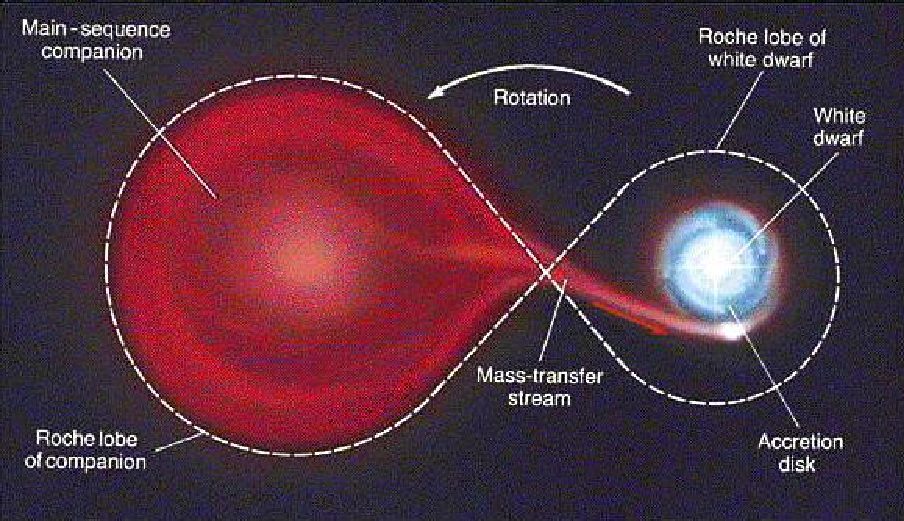
\includegraphics[scale=0.6]{images/lobederoche}
	\caption{Transfert de matière dans un système binaire et lobes de Roche}
\end{figure}\bigskip 

De plus en plus de matière commence donc à orbiter autour de la naine blanche, ce qui forme un disque d'accrétion autour de celle-ci. Ce disque, augmentant de masse, a pour effet d'accroître la pression et la température de l'étoile. Juste avant que la naine blanche n'atteigne la masse de Chandrasekhar 1,44 ($M_\odot$) % si elle avait été dépassée, alors la naine blanche se serait transformée en étoile à neutrons%
 , le carbone ainsi que l'oxygène se mettent à fusionner, chacun indépendamment, de manière anarchique. Comme le gaz composant l'étoile est dégénéré, la température peut donc croître extrêmement rapidement (§3.1.1). L'augmentation de température accélère la fusion chaotique de l'oxygène et du carbone. Par un phénomène encore mal compris et sujet à débat, l'étoile explose sous l'effet d'un ultime emballement des fusions thermonucléaires. Il ne reste plus rien après cette explosion, la matière s'éparpille dans le milieu interstellaire. \smallskip
 
 Les supernovas de type Ia sont les seuls supernovas thermonucléaires. Comme les types Ib et Ic, elles ne possèdent pas d'hydrogène dans leur spectre électromagnétique, cependant, contrairement à eux, on distingue la présence de raies de silicium dans sa composition. \bigskip
 
 \subsection{Nucléosynthèse lors d'une supernova} \medskip
 
 L'explosion d'une supernova permet de créer des éléments plus lourds que ceux produits lors d'une nucléosynthèse stellaire standard. Lors d'une supernova, un important flux de neutrons (10$^{20}$ neutrons cm$^{-2}$ s$^{-1}$) balaie les couches supérieures de l'étoile. Ces neutrons, ne possédant pas de charge électrique, peuvent être capturés par des atomes avoisinants grâce aux exceptionnelles conditions de pression et de température (T=10$^{9}$K et P=10$^{9}$ g cm$^{-3}$); ce phénomène s'appelle la capture de neutrons rapide, ou processus r. %note de bas de page processus s%
 Plus un atome capte des neutrons, plus il deviendra un grand isotope de cet élément. Le processus r s'arrête soit lorsque le noyau remplit toutes ses couches nucléaires et devient donc extrêmement stable, soit parce que le noyau est trop instable et est soumis à la radioactivité $\beta^{-}$. \smallskip
 Le noyau, lorsqu'il remplit toutes ses couches nucléaires, devient moins sensible aux réactions nucléaires. Remplir ses couches nucléaires signifient atteindre un nombre de nucléons égale à 20,28,50 ou encore 126. Ces nombres déterminé expérimentalement, pour lesquels un noyau atomique est très stable, sont aussi appelés nombres magiques. \smallskip 
 Si l'isotope devient instable, alors un neutron se dégrade en un proton, un électron et un antineutrino  par radioactivité $\beta^{-}$ (Eq. 3.3). \bigskip
 
\begin{equation} \ce{n -> \ce{p+} + \ce{e-} + $\overline{\nu}$_{e}} \end{equation} \bigskip
 
 Comme le noyau a gagné un proton, un nouvel élément est créé. Grâce à ce processus, des atomes tels que le plomb, l'or ou l'uranium peuvent être créer. Ce cycle peut se répéter tant que les conditions de flux neutronique, de pression et de température à la capture de neutrons sont remplies. Cependant, ces conditions ne sont remplies que pendant quelques secondes lors de l'explosion de la supernova. Tout ces éléments lourds sont par la suite répandus dans le milieu interstellaire à cause de l'explosion (§5). \bigskip
 
 \begin{figure}[H]
 	\centering
 	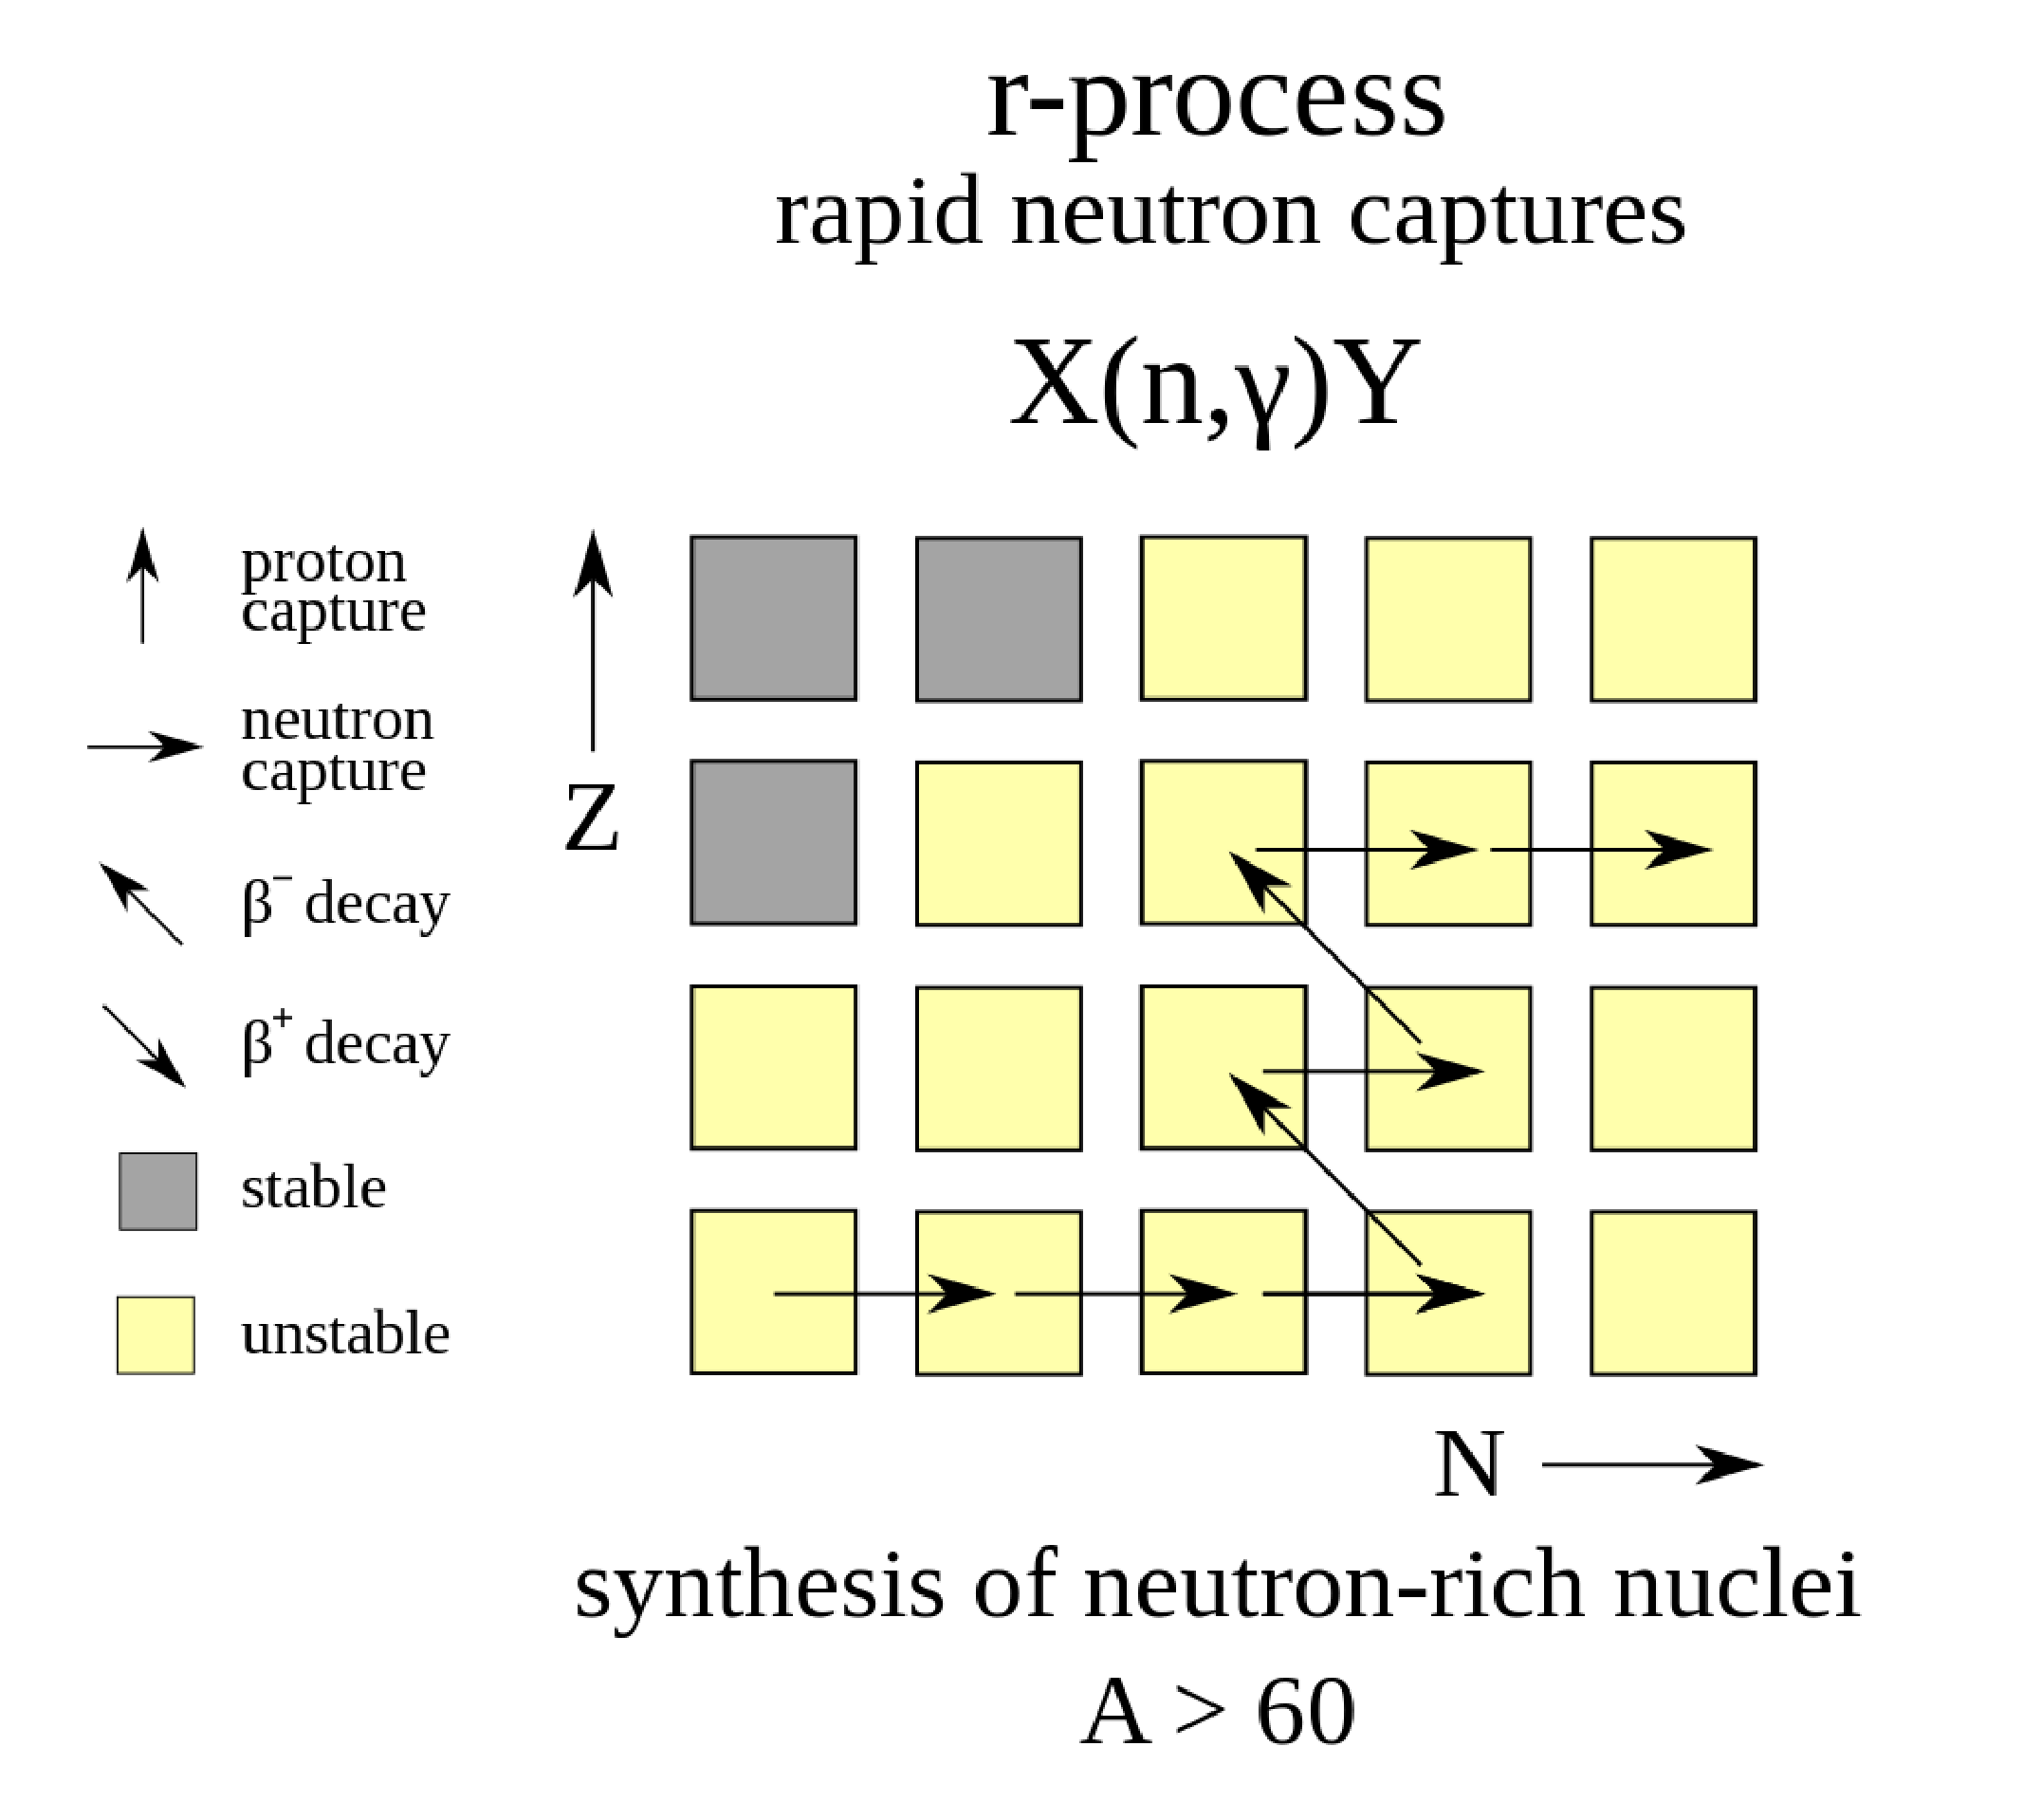
\includegraphics[scale=0.15]{images/processusr}
 	\caption{Trajectoire d'un atome capturant des neutrons dans le tableau périodique des éléments}
 \end{figure}\bigskip 
 
 
 



 
 

% !TeX encoding = UTF-8
% !TeX program = xelatex
% !TeX spellcheck = fr
% !TeX root = tm_astro_main.tex


\chapter{L'E-ELT}
% !TeX encoding = UTF-8
% !TeX program = xelatex
% !TeX spellcheck = fr
% !TeX root = tm_astro_main.tex

\chapterFormatfive

\chapter{Enrichissement du milieu interstellaire}\label{5}

\chapterFormat

Comme nous l'avons vu dans les chapitres \ref{2} et \ref{3}, des éléments lourds sont produits par les étoiles au cours de leur fin de vie. Ces éléments peuvent de différentes manières se retrouver séparés de leur étoile. Les vents stellaires incarnent l'une des ces manières; en effet les étoiles AGB (§\ref{2.2.2}) ainsi que les supergéantes (§\ref{2.4}) sont balayées par de forts vents parvenant à retirer jusqu'à plusieurs masses solaires de matière à l'étoile. Les nébuleuses planétaires (§\ref{2.3}) et les supernovas (§\ref{3}) représentent une autre méthode pour expulser dans le milieu interstellaire les composantes d'une étoile. Ces deux phénomènes mettent le coeur d'une étoile à nu; toute la matière qui constituait les anciennes couches supérieures de l'étoile est maintenant éjectée dans le vide interstellaire. 

\section{Evolution et rôle du milieu interstellaire}\label{5.1}

Au fil du temps, des nuages de gaz enrichis par la matière d'anciennes étoiles se forment: ce sont les nébuleuses. Ces objets célestes possèdent un rôle majeur dans la naissance des étoiles; on les surnomme d'ailleurs les pouponnières d'étoiles. Les composantes du gaz de la nébuleuse se rapprochent les uns des autres sous l'effet de la gravitation jusqu'à former une boule de gaz, nous disons que le gaz s'effondre. En même temps que la pression du gaz croît, la température augmente; arrive un certain stade où la température est suffisante pour déclencher la fusion de l'hydrogène, une nouvelle étoile est alors née. Autour de la jeune étoile se trouve toujours un nuage de gaz appelé disque protoplanétaire. A partir de celui-ci, des poussières interstellaires commencent à s'agréger. Les différents agrégats accrètent progressivement la matière du disque protoplanétaire. Au fur et à mesure, le disque disparaît en laissant place à des planètes, des comètes ou encore des astéroïdes. En fonction de la composition initiale du gaz, différentes planètes sont créées. Par exemple, dans le cas de notre système solaire, les planètes telluriques comme la Terre sont principalement constituées de silicium et de fer; Jupiter, quant à elle, est quasi intégralement composée d'hydrogène et d'hélium. De nos jours, nous savons donc que sans un milieu interstellaire enrichi par des générations entières d'étoiles, les éléments nécessaires à l'apparition de la vie n'auraient jamais été réunis. La célèbre citation de l'astrophysicien Hubert Reeves résume parfaitement cela: << On m'a dit: tu n'es que cendre et poussières. On a oublié de me dire qu'il s'agissait de poussières d'étoiles.>>

\begin{figure}[H]
	\centering
	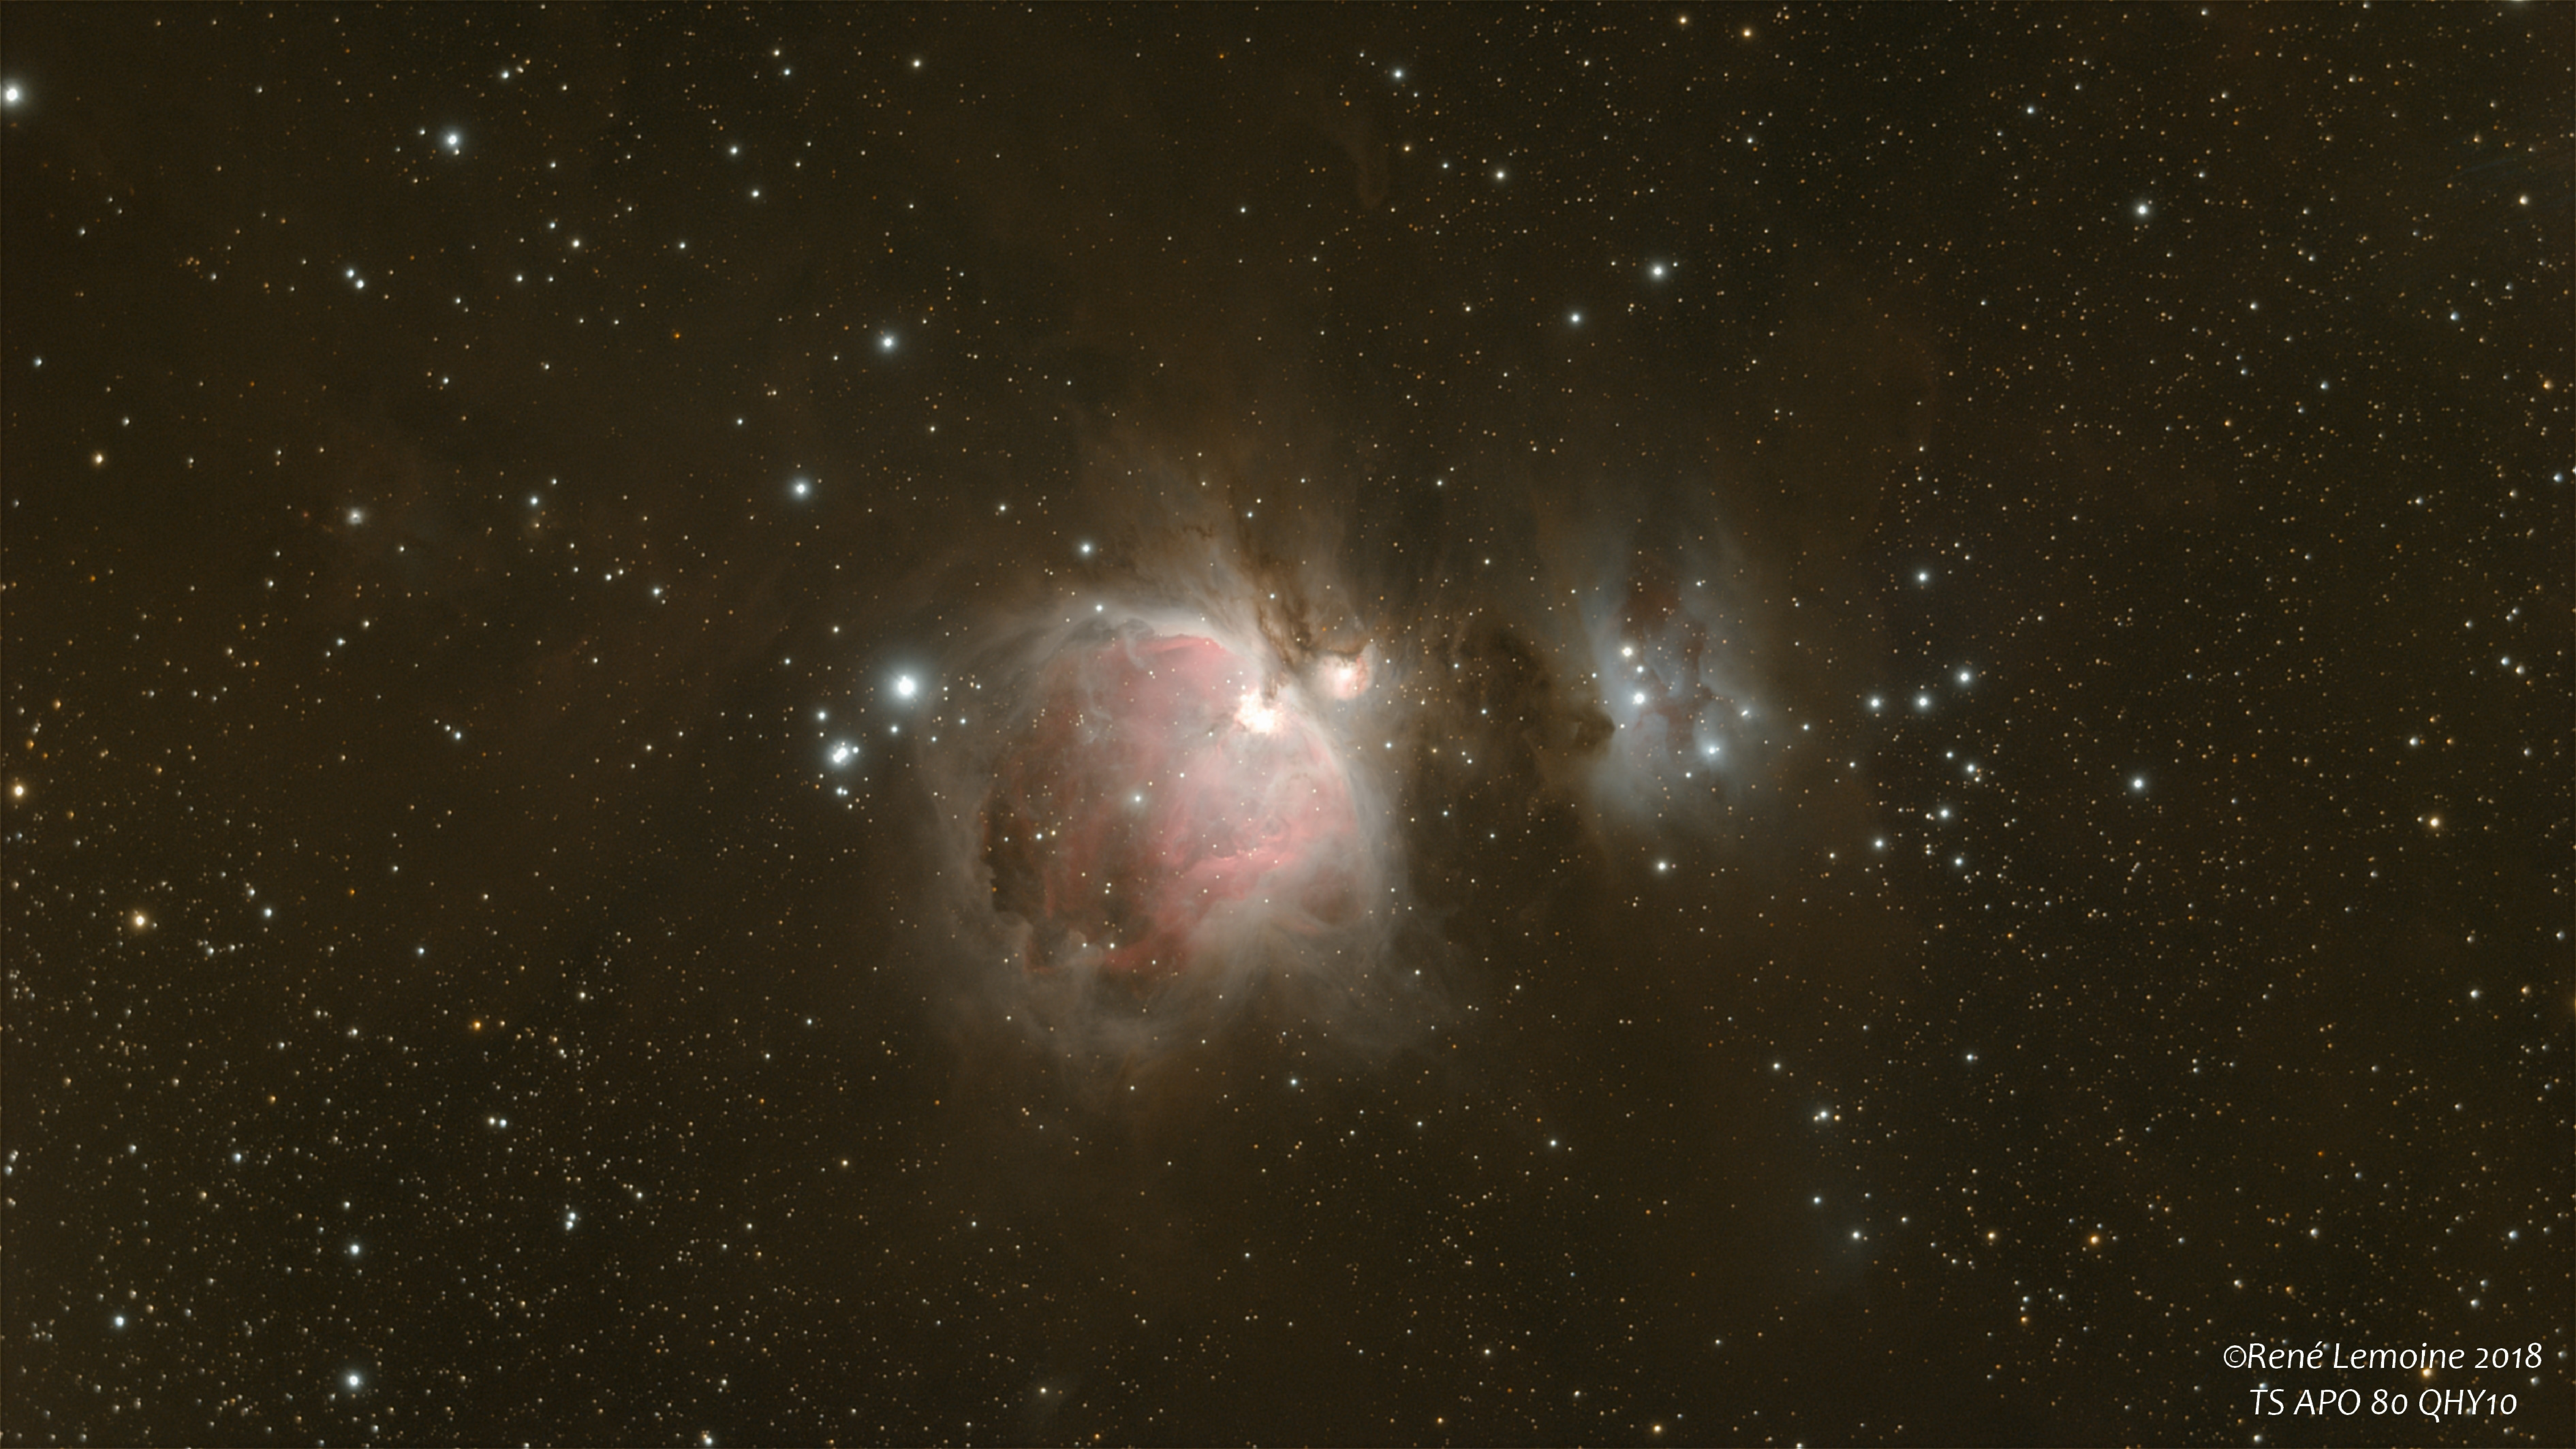
\includegraphics[scale=0.054]{images/orion}
	\caption[M42, nébuleuse d'Orion - astrophoto prise par René Lemoine en 2018 avec une lunette TS APO 80 et une caméra QHY10 (5 heures de pose)]{M42, nébuleuse d'Orion}
	\label{Fig. 5.1}
\end{figure}\bigskip



\section{ L'E-ELT dans ce domaine}\label{5.2}

Dans cette dernière section, nous allons traiter plus en profondeur des avancées attendues par l'E-ELT dans l'étude du milieu interstellaire. Dans un premier temps, nous nous attarderons plus spécifiquement sur l'observation de rémanent de supernova. Ensuite, comme nous avons déjà quelque peu parlé des exoplanètes dans la section \ref{5.1}, il convient de s'intéresser à leur observation par le télescope géant européen.\medskip

L'E-ELT sera particulièrement performant dans l'observation des supernovas de type Ia (§\ref{3.1.2}) à haut décalage vers le rouge. Ce type particulier est privilégié car une des caractéristiques principales des supernovas de type Ia est la présence de raies de silicium dans leur spectre électromagnétique (Annexe \ref{Annexe D}). Ce sera le spectrographe HARMONI (§\ref{4.2}), muni d'une optique adaptative, qui sera principalement chargé de cette mission. Le télescope géant européen révolutionnera ce domaine d'étude dans le mesure où il sera capable d'observer des décalages dans le rouge plus élevé que ceux aperçus avec d'autres télescopes déjà existant. Le fait que ces objets soient décalés vers le rouge signifie qu'ils s'éloignent de nous à grande vitesse; cela est dû à l'expansion de l'univers, qui de plus est accélérée. En d'autres termes, cela signifie que plus les objets sont distancés de nous, plus ils s'éloignent rapidement. De plus, comme la vitesse de la lumière est finie (299 792 $km/s$), tout ce que nous observons n'est pas réellement dans le présent, mais plutôt dans un passé plus ou moins lointain. Ainsi, si nous recombinons ce que l'on vient de dire, nous arrivons à la conclusion que plus on regarde décalé dans le rouge plus on regarde dans le passé. C'est grâce à ce phénomène que l'E-ELT aura la capacité d'observer des évènements qui se sont passés dans le premier dixième de la vie de notre univers. A titre d'information, les meilleurs télescopes à ce jour, dans le cadre de l'observation de supernovas, sont capables de "remonter" jusqu'à environ 70\% de l'âge de notre univers (supernova DES16C2nm observée en 2016). Il est intéressant de pouvoir analyser des évènements toujours plus éloignés dans le temps afin, d'une part augmenter notre niveau de compréhension de l'évolution primordiale de l'univers et, d'une autre part apporter de nouvelles pistes de compréhension aux théories traitant de sa création.\medskip

La recherche et l'étude des exoplanètes est l'un des principaux domaines de l'astronomie moderne. Ce secteur de recherche bénéficie d'un grand appui budgétaire, notamment grâce à ses objectifs scientifiques: la recherches de planètes potentiellement habitables et la découverte d'une possible vie extraterrestre. De nombreux télescopes ont pour objectif de découvrir, recenser ou encore analyser des exoplanètes. L'E-ELT ne déroge pas à cette règle avec son instrument HARMONI (§\ref{4.2}). Les télescopes existants qui étudient les exoplanètes utilisent principalement des techniques indirectes pour les détecter. Ces méthodes recherchent l'influence que possède une exoplanète sur son étoile hôte. Cette influence peut se manifester par des petites variations de luminosité (méthode des transits) ou bien encore par des variations de la vitesse radiale d'une étoile (méthode des vitesses radiales). Grâce à sa très grande résolution, l'E-ELT sera capable de tirer son épingle du jeu en observant directement certaines exoplanètes sans passer par des méthodes indirectes. De plus, son spectrographe aura la capacité d'identifier avec précision des molécules chimiques présentes dans des atmosphères d'exoplanètes relativement proches de nous. Dans notre quête de la découverte d'une vie extraterrestre, nous essayons de mettre la main sur des exoplanètes possédant les mêmes caractéristiques que la Terre. En détectant les mêmes molécules qui ont permis l'apparition de la vie sur notre planète (comme l'eau H$_{2} 0$) et en remplissant d'autres critères qui rendraient cette exoplanète semblable à la nôtre, il y aurait peut-être une infime chance qu'une forme de vie équivalente à la nôtre ait pu se développer. La limite de cette méthode se trouve dans le fait qu'en choisissant la Terre comme modèle de recherche, nous restreignons grandement le nombre de candidats pouvant abriter la vie. D'une certaine manière, la vie existe peut-être ailleurs, mais sous une forme bien différente de celle que nous imaginons.











% !TeX encoding = UTF-8
% !TeX program = xelatex
% !TeX spellcheck = fr
% !TeX root = tm_astro_main.tex


\chapter{Conclusion}
% !TeX encoding = UTF-8
% !TeX program = xelatex
% !TeX spellcheck = fr
% !TeX root = tm_astro_main.tex



\appendix

\chapter{Modèle polytropique}\label{Annexe A}

\begin{figure}[H]
	\centering
	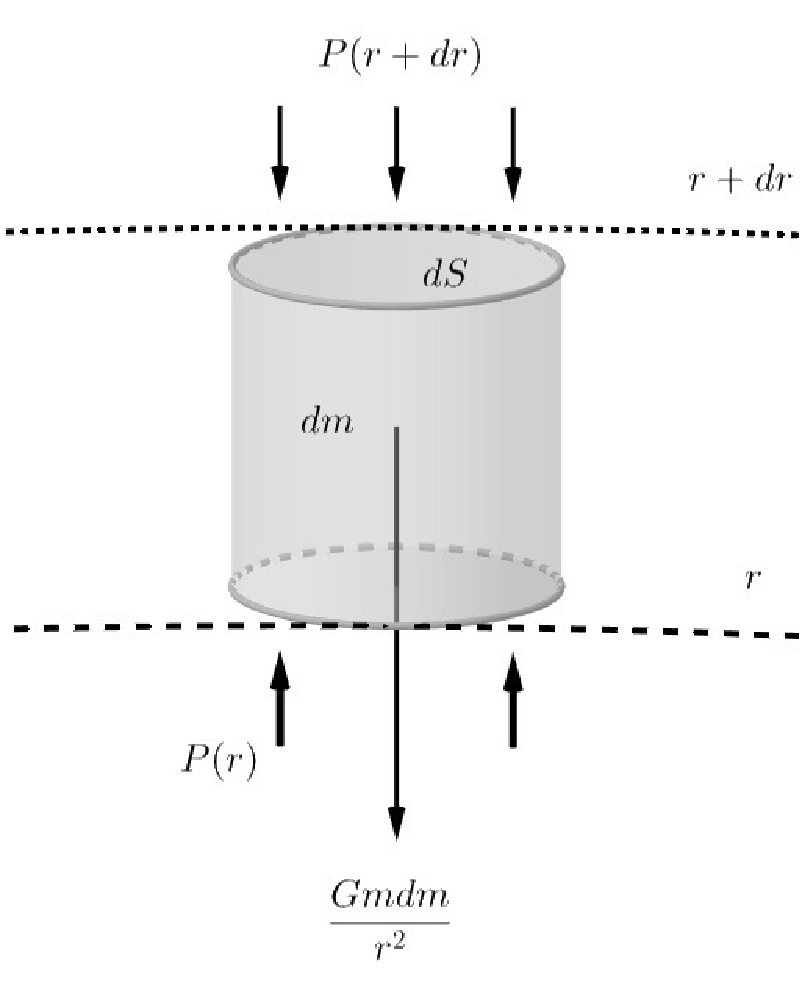
\includegraphics[scale=0.5]{images/cylindre}
	\caption[Cylindre de volume infinitésimal soumis à la force gravitationnelle et à la pression radiative - figure réalisée avec GeoGebra]{Cylindre de volume infinitésimal soumis à la force gravitationnelle et à la pression radiative}
	\label{Fig. A.1}
\end{figure}\bigskip

\begin{figure}[H]
	\centering
	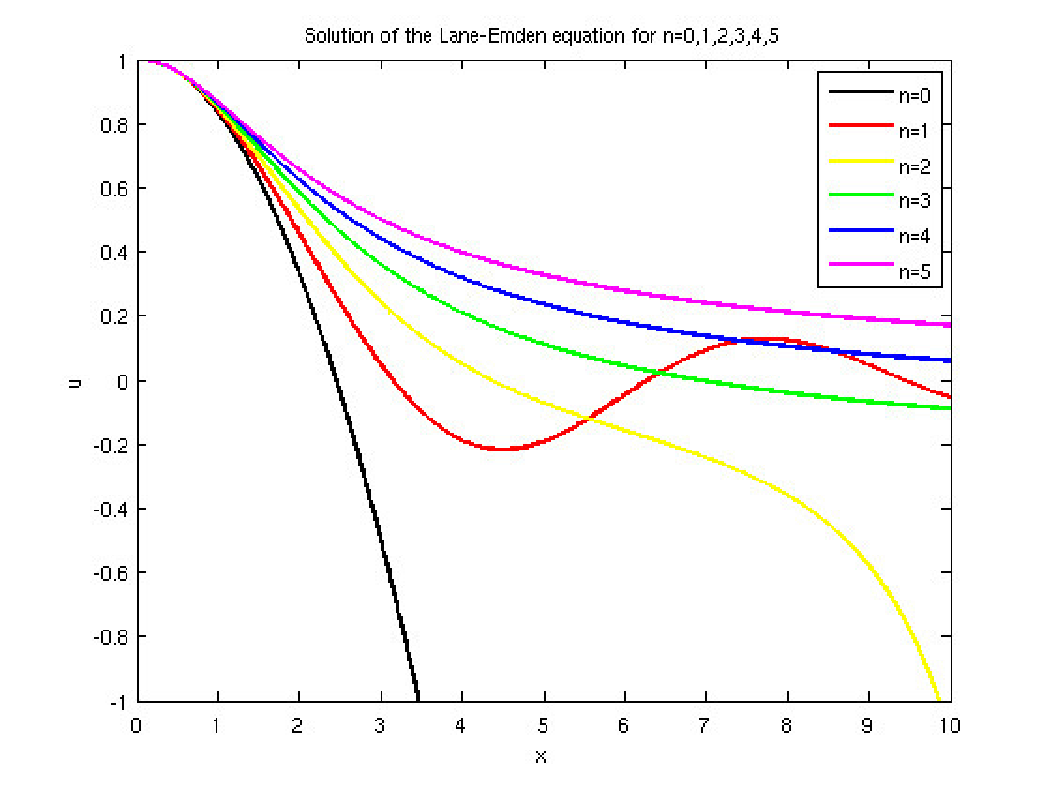
\includegraphics[scale=0.45]{images/graphe_poly}
	\caption[Valeurs de $\theta \left( \xi\right) $ en fonction de l'indice $n$ choisi]{Valeurs de $\theta \left( \xi\right) $ en fonction de l'indice $n$ choisi}
	\addloflink{https://www.mathworks.com/matlabcentral/mlc-downloads/downloads/submissions/23972/versions/22/previews/chebfun/examples/ode/html/LaneEmden.html}
	\label{Fig. A.2}
\end{figure}\bigskip


\chapter{Masse de Chandrasekhar}\label{Annexe B}

Dans les chapitre §\ref{2} et §\ref{3}, nous avons brièvement parlé de la masse de Chandrasekhar. Cette masse limite est la masse maximale que la pression de dégénérescence des électrons peut retenir sans que l'effondrement gravitationnel se poursuive. Elle a été découverte et calculée en 1930 par le physicien indien Chandrasekhar.  Grâce au modèle polytropique que nous avons développé au §\ref{1.2}, nous allons pouvoir obtenir la valeur numérique de cette fameuse limite.\bigskip

Tout d'abord, isolons $\rho_c$ dans l'Eq. \ref{Eq. 1.17}, remplaçons ce résultat dans l'Eq. \ref{Eq. 1.22},  dans cette même équation substituons $\alpha$ par l'Eq. \ref{Eq. 1.20} et réarrangeons les termes, nous obtenons: \begin{equation}\left( \dfrac{GM}{M_{n}}\right)^{n-1} \left( \dfrac{R}{R_{n}}\right)^{3-n}=\dfrac{\left[ \left( n+1\right)K\right]^n}{4\pi G}\label{Eq. 7.1}\end{equation}
avec arbitrairement choisis:
\begin{equation}M_{n}=-\xi_{1}^{2}\left( \dfrac{d\theta}{d\xi}\right)_{\xi_{1}}\label{Eq. 7.2}\end{equation}

\begin{equation}R_{n}=\xi_{1}\label{Eq. 7.3}\end{equation}

De plus, dans l'Eq.\ref{Eq. 7.1}, pour la valeur $n=3$, la masse $M$ est uniquement déterminée par $K$ et indépendante du rayon $R$: 
\begin{equation}M=4\pi M_{3}\left(\dfrac{K}{\pi G}\right)^{3/2}\label{Eq. 7.4}\end{equation}

Ensuite, si $1<n<3$, nous avons de l'Eq.\ref{Eq. 7.1}:
\begin{equation}R^{3-n}\propto\dfrac{1}{M^{n-1}}\label{Eq. 7.5}\end{equation} L'Eq. \ref{Eq. 7.5} nous dit que plus la masse d'un noyau stellaire augmente, plus son rayon diminue.\smallskip 

Nous essayons ici donc de trouver le noyau le plus massif et donc le plus dense qui soit encore en équilibre thermodynamique (§\ref{1.1}); la masse que possède le noyau que nous cherchons est la masse de Chandrasekhar.\smallskip

Le cas limite d'un gaz, composant une étoile, soumis à une énorme pression engendrée par une densité extrême est un gaz relativiste dégénéré. Nous le qualifions de relativiste, car les particules qui le composent sont soumises à de tels niveaux de pression qu'elles atteignent presque la vitesse de la lumière.\smallskip

L'équation d'état polytropique (Eq. \ref{Eq. 1.13}) décrivant ce type de gaz est donné par:\begin{equation}P=K_{2}  \rho^{4/3}\label{Eq.7.6}\end{equation}
avec $K_{2}$ étant déterminé par des lois quantiques et relativistes \autocite{prialnikIntroductionTheoryStellar2009}:
\begin{equation}K_{2}=\dfrac{hc}{8}\left(\dfrac{3}{\pi}\right)^{1/3} \dfrac{1}{m_{H}^{4/3}}\hspace{5pt}\mu_e^{-4/3}\label{Eq. 7.7}\end{equation}
A partir de l'indice adiabatique $\gamma = 4/3$, il est aisé de déterminer l'indice polytropique (Eq. \ref{Eq. 1.14}): $n=3$. De plus, l'Eq. \ref{Eq. 7.4} nous a permis de montrer que pour $n=3$, la masse $M$ est uniquement dépendante de $K$; autrement dit, pour un $K$ donné, il existe une seule masse $M$ possible. Ainsi, si nous substituons $K$ par $K_{2}$ (décrivant le cas limite d'un gaz dégénéré relativiste) dans l'Eq. \ref{Eq. 7.4}, nous obtenons la masse limite de Chandrasekhar: \begin{equation}M_{Ch}=\dfrac{M_{3}\sqrt{1.5}}{4\pi}\left( \dfrac{hc}{Gm_{H}^{4/3}}\right)^{3/2}\hspace{5pt}\mu_{e}^{-2}\label{Eq. 7.8}\end{equation}

En insérant la valeur des constantes l'expression se transforme en:
\begin{equation}M_{Ch}=5.83\hspace{3pt}\mu_{e}^{-2}M_\odot\label{Eq. 7.9}\end{equation}

La variable $\mu_{e}$ décrit la composition chimique d'une étoile. Si le coeur d'une étoile est composé de fer: $\mu_{e}=2.15$; si il est composé de carbone et d'oxygène: $\mu_{e}=2$. La masse de Chandrasekhar n'est donc pas une valeur fixe, elle peut varier un peu en fonction des constituants de l'étoile.\bigskip

Pour $\mu_{e}=2$: 
\begin{equation}M_{Ch}=1.46\hspace{3pt}M_\odot\label{Eq. 7.10}\end{equation}

\chapter{Durée de vie des étoiles}\label{Annexe C}
\vspace{1cm}
\begin{figure}[H]
	\centering
	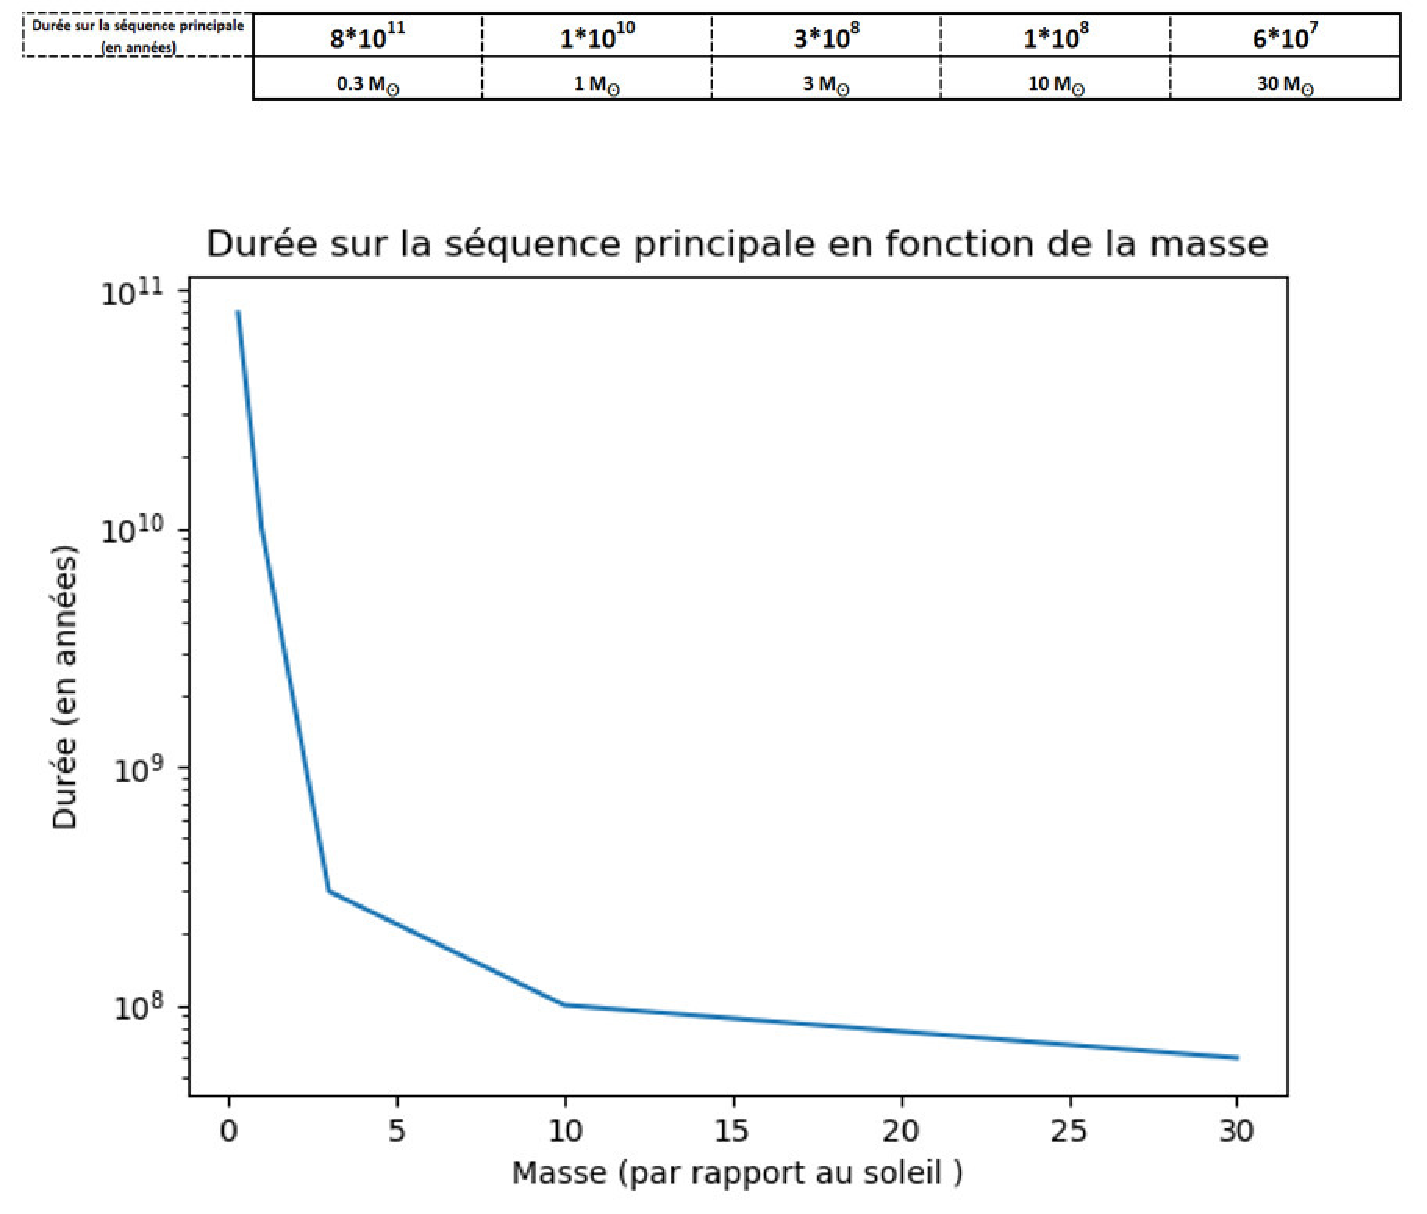
\includegraphics[scale=0.65]{images/duree}
	\caption[Durée de vie d'une étoile en fonction de sa masse - figure réalisée avec Matplotlib]{Durée de vie d'une étoile sur la séquence principale en fonction de sa masse}
	\label{Fig. C.1}
\end{figure}\bigskip

Le graphe ci-dessus nous montre une relation étonnante: la durée de vie d'une étoile est inversement proportionnelle à sa masse . Cela peut s'expliquer par le fait que chaque étoile conserve son équilibre hydrostatique tout au long de la séquence principale. En effet, pour qu'une étoile atteigne l'équilibre hydrostatique, la force gravitationnelle doit être exactement compensée par la force radiative . Ainsi, plus l'étoile est massive, plus la force radiative devra être grande, plus le "carburant" de l'étoile s'épuisera rapidement et précipitera la mort de celle-ci.



\chapter{Spectres électromagnétiques}\label{Annexe D}
\vspace{1.5cm}
\begin{figure}[H]
	\begin{minipage}[width=5cm]{.46\linewidth}
		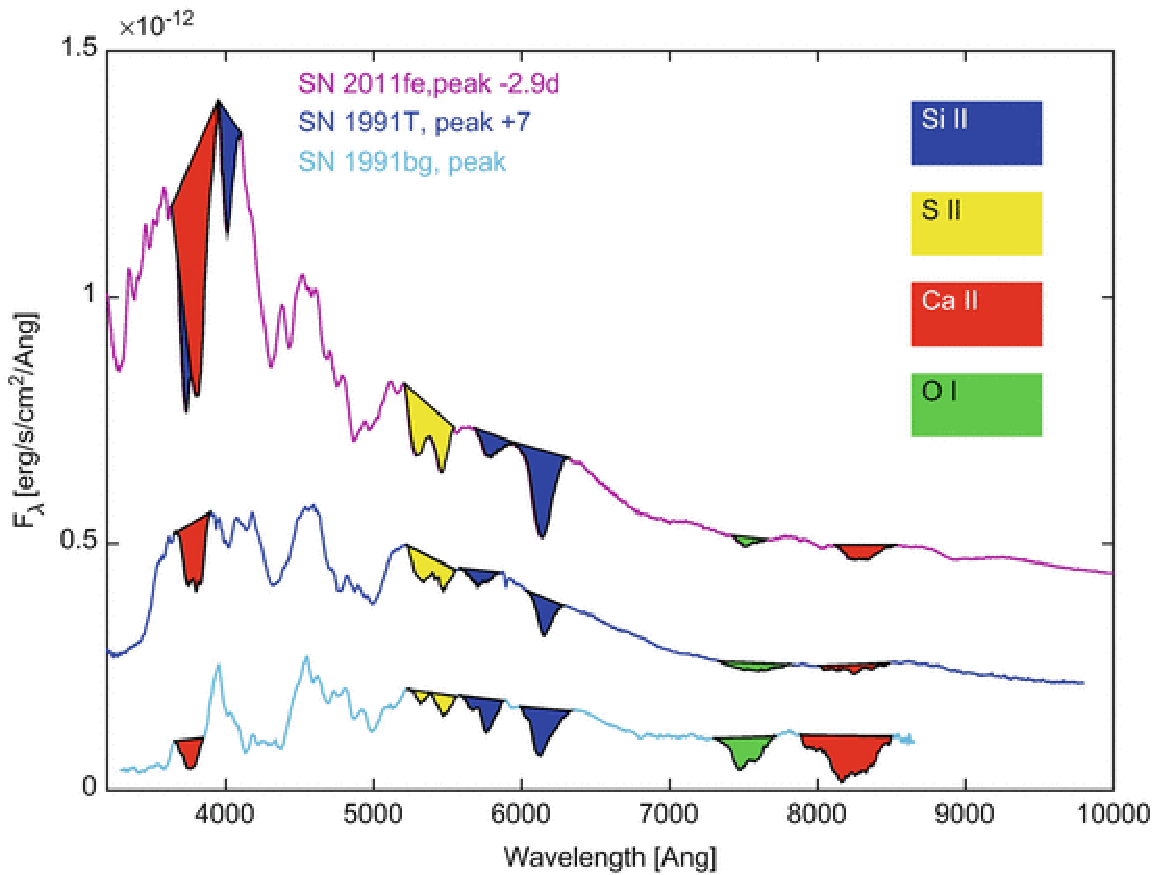
\includegraphics[scale=0.40]{images/1a}
	\end{minipage} \hfill
	\begin{minipage}[width=5cm]{.46\linewidth}
		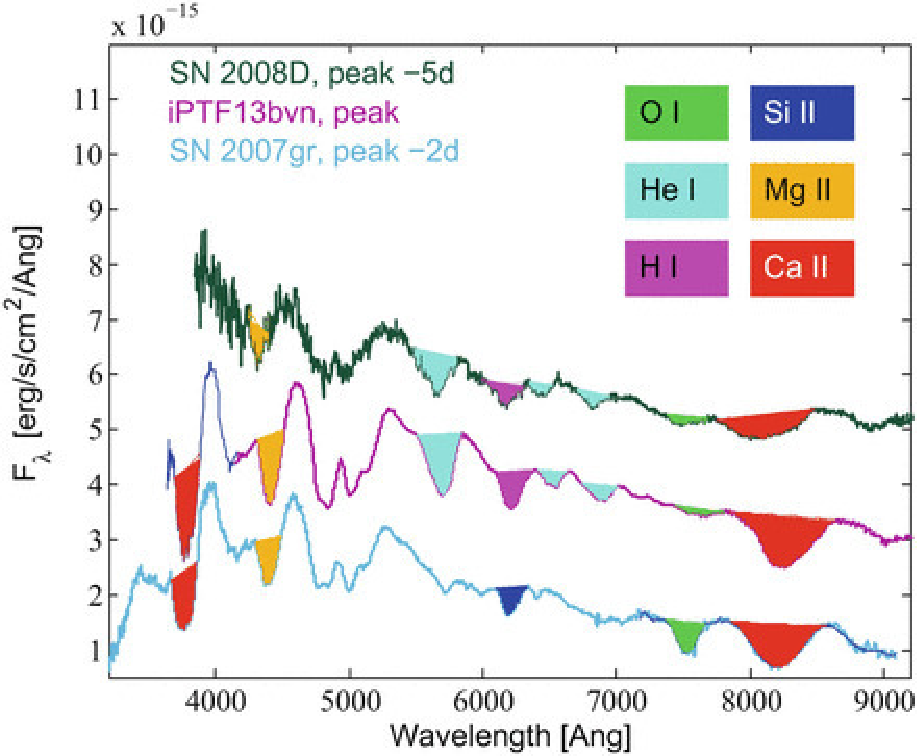
\includegraphics[scale=0.50]{images/1b}
	\end{minipage}
	\caption[Spectres de supernovas de type Ia et Ib]{Spectres de supernovas de type Ia (à gauche) et Ib (à droite): Le type Ia se caractérise par la présence de silicium, tandis que le type Ib se distingue par l'existence de raies d'hélium.}
	\addloflink{https://link.springer.com/referenceworkentry/10.1007\%2F978-3-319-20794-0_35-1}
\end{figure}

\vfill

\begin{figure}[H]
	\begin{minipage}[width=5cm]{.46\linewidth}
		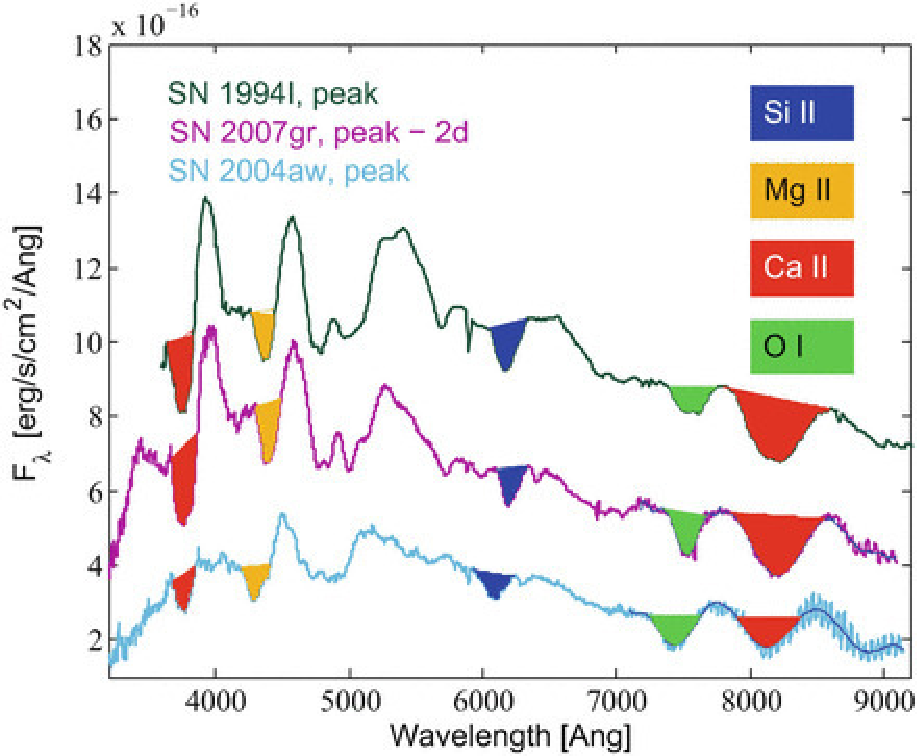
\includegraphics[scale=0.49]{images/1c}
		\caption[Spectre de supernova de type Ic]{Spectre de supernova de type Ic: absence d'hélium et d'hydrogène}
		\addloflink{https://link.springer.com/referenceworkentry/10.1007\%2F978-3-319-20794-0_35-1}
	\end{minipage} \hfill
	\begin{minipage}[width=5cm]{.46\linewidth}
		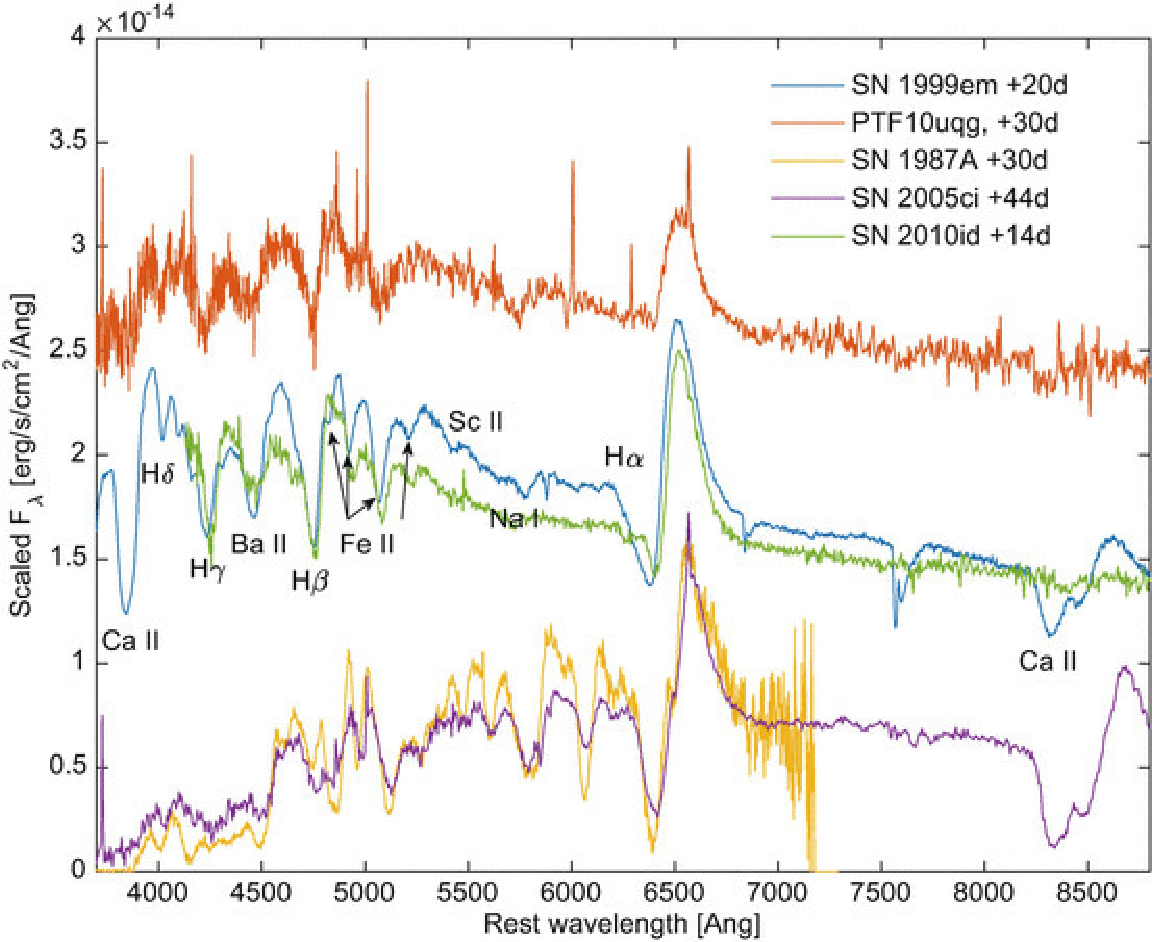
\includegraphics[scale=0.40]{images/2}
		\caption[Spectre de supernova de type II]{Spectre de supernova de type II: grande présence d'hydrogène}
		\addloflink{https://link.springer.com/referenceworkentry/10.1007\%2F978-3-319-20794-0_35-1}
	\end{minipage}
\end{figure}







\nocite{esslingerSupergeantes}
\nocite{comtegeorgesSyntheseElementsChimiques}
\nocite{esslingerGeantesRouges}
\nocite{esslingerNebuleusesPlanetaires}
\nocite{prialnikIntroductionTheoryStellar2009}
\nocite{audouzeAstrophysiqueNucleaire2003}
\nocite{branchSupernovaExplosions2017}
\nocite{bouquetINTRODUCTIONAUXSUPERNOVAE}
\nocite{FaconVivrePropre}
\nocite{courbinfredericPolycopieAstroIEPFL}
\nocite{EquationEtatInterieur}
\nocite{petriPhysiqueStellaire}
\nocite{prof.shudemaoStellarEquationPdf}
\nocite{dr.balsaterzicLecture23Pdf}
\nocite{informationeso.orgExtremelyLargeTelescope}
\nocite{TelescopeGeantEuropeen2019}
\nocite{brissonELTDerniereGeneration2017}
\nocite{hugotPolissageSousContraintes2015}
\nocite{informationeso.orgFirstInstrumentsEELT}
\nocite{MasseChandrasekhar2019}

\printbibliography

\listoffigures

\end{document}
